\documentclass[11pt]{article}
\usepackage[a4paper,margin=2.35cm]{geometry}
\usepackage{amsmath,amssymb,amsthm,mathtools,bm}
\usepackage{booktabs,tabularx,longtable,array}
\usepackage{graphicx}
\usepackage{xcolor}
\usepackage{microtype}
\usepackage{hyperref}
\usepackage{enumitem}
\usepackage{placeins}
\usepackage[numbers,sort&compress]{natbib}
\setlength{\emergencystretch}{2em}
\hypersetup{colorlinks=true,linkcolor=blue!45!black,citecolor=blue!45!black,urlcolor=blue!45!black}

\newtheorem{definition}{Definition}
\newtheorem{proposition}{Proposition}
\newtheorem{theorem}{Theorem}
\newtheorem{lemma}{Lemma}
\newtheorem{corollary}{Corollary}
\newtheorem{remark}{Remark}
\newcommand{\cH}{\mathcal H}
\newcommand{\cM}{\mathcal M}
\newcommand{\cQ}{\mathcal Q}
\newcommand{\cE}{\mathcal E}
\newcommand{\Tr}{\operatorname{Tr}}
\newcommand{\Desc}{\operatorname{Desc}}

\title{\textbf{Quantum Readout from Observer-Relative Lossy Descent}\\
\large Tau Core Foundation Paper VI: A finite conditional quantum terminal}
\author{Jozsef Olcsak}
\date{August 2026}

\begin{document}
\maketitle

\begin{abstract}
We ask which additional structures are required for an observer-relative,
information-losing descent from an atemporal morphological body to support a
quantum terminal rather than ordinary classical coarse graining.  First, a
finite countermodel proves that resolution loss, non-injectivity and stable
record classes alone imply neither complex amplitudes nor interference, Born
probabilities, entanglement or no-signalling.  We then state a finite
conditional source packet.  A positive quotient metric and a compatible
nondegenerate two-form construct a complex Hilbert carrier when the associated
endomorphism has one common complex scale.  A commuting self-adjoint generator
gives unitary transport; positive normalized effects give the trace Born rule;
and an explicitly selected tensor product gives local-CPTP no-signalling.

Inside an adopted enriched Tau completion, these structures are represented
on one normalized complex matrix block with a common action unit.  We prove
finite record-separation and tensor-factorization criteria, distinguish exact
logical recovery from dephasing, and give an approximate-recovery bound.  The
standard free algebraic-QFT and perturbative causal-QFT constructions are used
only as conditional fixed-background limits.  None of these standard quantum
results is presented as a Tau-specific deviation.

The proposed discriminator instead compares two independently reconstructed
quantities on the same occupied record pair: a normalized body-action
separation and its Uhlmann chord.  The completion requires them to agree, with
a certified recovery-error envelope.  A public-data audit finds no carrier on
which the action-side quantity is independently observable, so the
discriminator is not yet executable.  We also prove that the present narrow
base--seed reduct does not select the full joint source packet.  Consequently
the paper establishes a mathematically explicit conditional quantum terminal,
not a quantum theory derived from the unrestricted physical parent law; it
does not derive the SI value of
$\hbar$, physical outcome selection, nonperturbative QFT, quantized geometry or
the Standard Model.
\end{abstract}

\begin{center}
\fbox{\begin{minipage}{0.92\linewidth}
\textbf{Dependency and ownership.}
Inputs are: the atemporal body and observer-access architecture (Paper I),
typed finite source support (Paper II), recovery-correctable record transport
(Paper III), the common-source occupation boundary (Paper IV), and stable
observer quantization plus a calibrated terminal clock (Paper V).  This paper
owns the loss-only no-go, the finite metric--symplectic quantum completion,
Born/interference and no-signalling terminals, and the quantum/classical
status ledger. It also owns the recovery-based factor selector, its
approximate error bound and the central-chirality terminal-blindness theorem.
It neither re-proves nor silently strengthens its inputs.  The downstream
scalar-15/type-II mass and RG specialization is owned by Paper VII-C; it does
not replace the observer quantizer or the quantum source packet proved here.
\end{minipage}}
\end{center}

\begin{center}
\fbox{\begin{minipage}{0.92\linewidth}\small
\textbf{Atemporal parent-realization terminology.}
Because the Tau parent is atemporal, phrases such as ``Nature selects'' do
not denote an external agent or a later choice.  Their precise meaning is the
internal physical implication
\[
 (B_\tau^{\rm phys},s_U,\mathcal L_{\rm parent})
 \Longrightarrow \mathfrak P,
\]
together with occupation of the support of the resulting packet
$\mathfrak P$.  A theorem inside a declared completion proves only
class-relative realization.  It does not prove this unrestricted base--seed
arrow, and agreement of finitely many terminal readouts cannot by itself
establish ambient-source exhaustivity.  Current-facing statements therefore
use \emph{parent-law realization} and \emph{physical occupation}; any retained
legacy selection language is shorthand for this same distinction.
\end{minipage}}
\end{center}

\section{Inherited proof hierarchy}

Paper VI is a consolidation and terminal-recovery paper, not a restart of the
quantum branch.  A corpus-wide audit of the theory hub and Papers I--V gives
the following inherited ladder.

\begin{table}[h]
\centering
\small
\begin{tabularx}{\linewidth}{>{\raggedright\arraybackslash}p{0.19\linewidth}>{\raggedright\arraybackslash}p{0.36\linewidth}X}
\toprule
Level & Inherited result & Status used here \\
\midrule
Algebraic & A full-role operator square
$C(v)^2=K_*(v,v)I$ polarizes to the Clifford relations & Exact implication \\
Representation & Seven P3 generators admit the finite packet
$\mathrm{Cl}_7(\mathbb C)\simeq M_8(\mathbb C)\oplus M_8(\mathbb C)$ &
Constructed conditional representation \\
Completion & The graph-normal P3 handoff realizes the operator square with
one action unit and zero body Schur remainder & Adopted minimal post-body
completion \\
Record/terminal & Full S4 effects and the S5 square-root terminal supply the
sharp spectral instruments; the matrix block supplies metric, phase, unitary
and Born structures & Conditional recovery inside the enriched MVP \\
Field limit & Globally hyperbolic descent, Hadamard preparation and local
causal factorization supply free and perturbative interacting QFT structure &
Conditional standard recovery; interaction content and nonperturbative limit open \\
Physical source & The current narrow parent has no typed full-role incidence
into the squared-Hodge carrier & Exact current-source no-entailment;
unrestricted enriched-packet occupation open \\
\bottomrule
\end{tabularx}
\caption{Inherited proof hierarchy.  The open top-level source arrow does not
erase the lower-level theorems, while the lower-level constructions do not
prove unrestricted physical occupation.}
\label{tab:inherited}
\end{table}

This hierarchy fixes the interpretation of the paper.  The mathematical P3
and quantum-terminal machinery is already available at several levels.  The
remaining source question is the typed incidence
\begin{equation}
 \iota_{P3}:(E_{P3},K_*)\longrightarrow
 (R_{\rm common},h_{\rm common}),
 \label{eq:p3incidence}
\end{equation}
selected before the handoff.  Existing EACER support is rank two; the
rank-nine seed-normal and endpoint/context carriers lack the required typed
map; and the common Clifford envelope is an operator target rather than the
source incidence.  Paper VI uses the adopted completion for forward terminal
theorems and keeps Eq.~\eqref{eq:p3incidence} open at the unrestricted
physical parent-law level.

\section{Question, architecture and claim boundary}

Let $M_\tau$ denote a stabilized atemporal morphological body generated by the
physically enriched Tau base and a universal seed.  For an observer carrier
$O$, source region $S$ and context $c$, the accessible terminal information is
not the body itself.  It is obtained through a body-conditioned relation and a
stable finite-resolution map,
\begin{equation}
 B_\tau^{\rm phys}+s_U\longrightarrow M_\tau
 \longrightarrow \mathcal C_{OS|c}(M_\tau)
 \xrightarrow{Q_{OS|c}}\mathcal R_{OS|c}.
 \label{eq:spine}
\end{equation}
Here $\mathcal C_{OS|c}$ is not a separate substance.  It is the
observer--source realization of relations already conditioned by the body.
The stable quantizer $Q_{OS|c}$ defines observer-relative readout classes.
Equality of classes, rather than a non-transitive distance threshold, defines
the operational equivalence relation
\begin{equation}
 x\sim_{OS|c}y\quad\Longleftrightarrow\quad
 Q_{OS|c}(x)=Q_{OS|c}(y).
 \label{eq:equivalence}
\end{equation}

The central question is finite and deliberately narrow:
\begin{quote}
Which additional source-owned structures turn the quotient
$\mathcal C_{OS|c}/\!\sim_{OS|c}$ into a complex quantum carrier, and which
familiar quantum laws then follow without further fitted gains?
\end{quote}

Figure~\ref{fig:spine} displays the complete logical direction.  In
particular, terminal observations constrain a frozen forward construction;
they do not ontologically build $M_\tau$ backwards.

\begin{figure}[t]
\centering
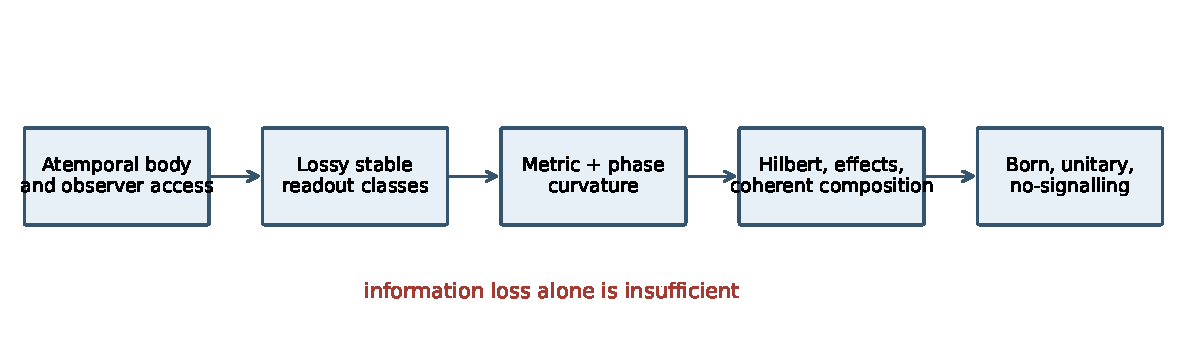
\includegraphics[width=0.96\linewidth]{../figures/fig_quantum_descent_spine.pdf}
\caption{The Paper-VI descent.  Finite resolution supplies stable classes,
whereas complex phase geometry, effects and composition require additional
source-owned structure.  Dashed implications are conditional.}
\label{fig:spine}
\end{figure}

\section{Relation to established structures and novelty boundary}

The terminal mathematics used below is standard once its inputs are granted.
Stinespring/Kraus theory supplies completely positive channels
\citep{Stinespring1955,Kraus1971}; Lindblad dynamics supplies a standard
decoherence limit \citep{Lindblad1976}; Uhlmann geometry supplies mixed-state
purification distance \citep{Uhlmann1976}; Gleason-type results constrain
noncontextual probability measures \citep{Gleason1957}; and quantum error
correction supplies exact recoverability criteria
\citep{KnillLaflamme1997,Petz1986}.  Quantum-geometric response and speed-limit
relations are likewise established structures
\citep{Kolodrubetz2017Geometry,AnandanAharonov1990}.  Paper VI does not claim
these results as new consequences of information loss.

The novelty claim is narrower and conditional.  Tau Core asks whether one
body-derived, observer-relative source packet can own the metric, phase,
action unit, effects, subsystem composition and recovery domain together,
rather than importing them as unrelated terminal axioms.  The paper gives
finite sufficient conditions, countermodels to weaker packets and one proposed
cross-domain discriminator.  It does not prove that the physical base--seed
system occupies the sufficient packet.  This distinction separates the
paper's source-architecture proposal from its use of standard quantum and QFT
theorems.

\section{The common accessibility quotient}

\begin{definition}[Stable observer quantizer]
A stable observer quantizer is an idempotent measurable map
$Q_{OS|c}:\mathcal C_{OS|c}\to\mathcal R_{OS|c}$ whose fibres form a
partition on the occupied source family and remain invariant under the
declared record-tolerance class.  Its finite capacity is the number, measure
or effective dimension of occupied distinguishable fibres.
\end{definition}

This definition retains observer dependence.  Different carriers, source
supports or contexts may induce different partitions.  Microscopic effective
discreteness and macroscopic effective continuity can therefore coexist: a
fine carrier resolves fewer equivalence identifications, while redundant
compatible records make a dense family of transitions operationally smooth.

For an ordered source path $\gamma$, time quantization is the smallest ordered
transition whose endpoints occupy distinct stable fibres.  It is not a
universal atom of time unless independence from $O,S,c$ is proved.  Likewise,
multiple parent configurations in one ordinary class are merely unresolved;
they are not yet a coherent superposition.

\section{Loss-only no-go}

\begin{proposition}[Loss-only no-go]
\label{prop:nogo}
Finite capacity, non-injectivity and a stable ordered quotient do not imply a
complex Hilbert space, phase-sensitive composition, the Born rule,
entanglement or no-signalling.
\end{proposition}

\begin{proof}
Take the reported state space to be the classical bit simplex $\Delta_2$.  One
completion is $\Delta_2$ itself with stochastic maps.  A second completion is
the qubit density-operator space followed by complete dephasing in a fixed
basis,
\begin{equation}
 \mathcal D(\rho)=\operatorname{diag}(\rho)\in\Delta_2.
\end{equation}
Both have exactly the same resolved quotient, occupied probability states and
finite outcome alphabet.  Before dephasing, the quantum completion also has
off-diagonal phase and interference, whereas the classical completion does
not.  Adding the same order to the two reported outcomes changes neither
construction.  Hence the common loss/quotient data cannot select any of the
listed quantum properties.
\end{proof}

This no-go protects the program from an otherwise tempting circularity.  It
also explains why observer-dependent quantization is necessary but not
sufficient.  Figure~\ref{fig:fork} summarizes the fork.

\begin{figure}[t]
\centering
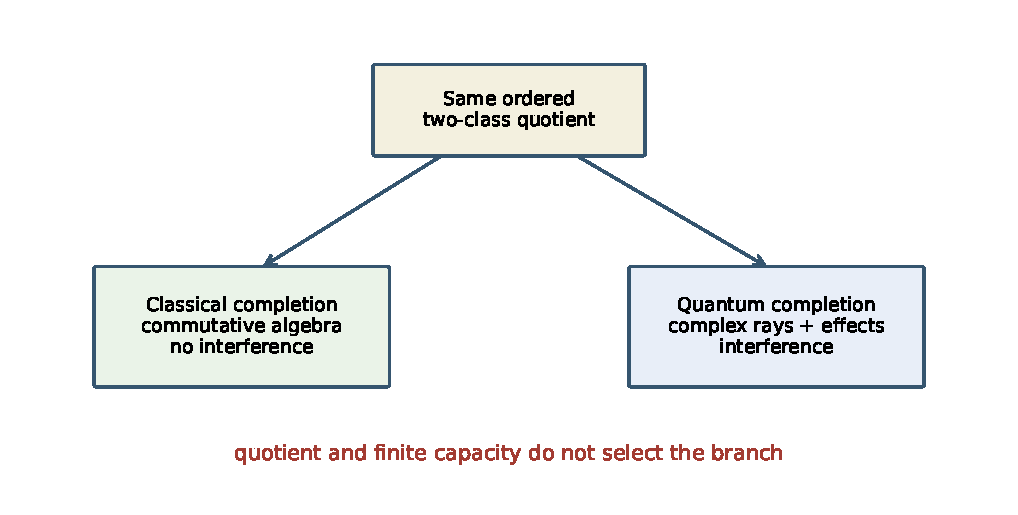
\includegraphics[width=0.88\linewidth]{../figures/fig_quantum_classical_fork.pdf}
\caption{The same finite observer quotient admits a classical simplex and a
complex quantum carrier.  The distinguishing datum is phase-capable coherent
composition, not information loss by itself.}
\label{fig:fork}
\end{figure}

\section{Frozen quantum source packet}

We now state the smallest packet used in the positive construction.  Every
item must arise from one frozen post-body source; the packet may not be
assembled by fitting terminal residuals.

\begin{definition}[Quantum source packet]
On an occupied finite-dimensional horizontal tangent space $V_O$, let
\begin{equation}
 \mathfrak P_Q=(g,\theta,\omega,U_A,K,\mathfrak E,\otimes),
 \qquad \omega=d\theta,
 \label{eq:packet}
\end{equation}
where:
\begin{enumerate}[label=(Q\arabic*)]
\item $g$ is the positive quotient of the body Hessian;
\item $\theta$ is a source-owned ordered-action one-form and $\omega$ its
nondegenerate curvature on the quantum leaf;
\item $A=g^{-1}\omega$ obeys $A^2=-\kappa^2 I$ for one $\kappa>0$;
\item $U_A>0$ is the common action unit, with no block-dependent gain;
\item $K$ is $g$-self-adjoint and commutes with $J=A/\kappa$;
\item $\mathfrak E$ is a normalized positive effect family represented by the
source-owned trace state;
\item $\otimes$ is a declared composition law on independently accessible
occupied subsystems, and local deterministic operations are CPTP.
\end{enumerate}
\end{definition}

Items (Q1)--(Q3) are the metric--symplectic completion.  Items (Q4)--(Q6)
select dynamics and readout statistics.  Item (Q7) is logically independent:
no-signalling cannot be proved before a subsystem composition is defined.

\section{Existing Tau source realization}

The packet can now be evaluated against earlier Tau source results rather
than left as a free list.  Inside the declared source-irredundant enriched
MVP, the existing occupation theorem supplies an occupied coherent P3
representation and a faithful record edge.  The adopted graph-normal P3
handoff has stationary operator coordinate
\begin{equation}
 S_{P3}=c_K(e_{P3})
\end{equation}
in the complex Clifford carrier, with one action unit $\mathcal A_*$ and the
normalized trace.  Its finite source-minimal block ledger is
\begin{equation}
 \mathrm{Cl}_7(\mathbb C)\simeq
 M_8(\mathbb C)\oplus M_8(\mathbb C).
 \label{eq:cl7}
\end{equation}

Restrict to one occupied simple block $\mathcal A_Q=M_n(\mathbb C)$ and let
$\tau_n=\Tr/n$.  On $\mathcal A_Q$ define
\begin{equation}
 h(X,Y)=\mathcal A_*\tau_n(X^\dagger Y),\quad
 g=\operatorname{Re}h,\quad JX=iX,\quad
 \omega(X,Y)=g(JX,Y).
 \label{eq:matrixpacket}
\end{equation}
Because the matrix block is an affine vector space, the canonical linear
potential
\begin{equation}
 \theta_X(Y)=\frac12\omega(X,Y)
 \label{eq:matrix-phase-potential}
\end{equation}
satisfies $d\theta=\omega$.  Thus the construction supplies the one-form in
(Q2), not only its curvature.

\begin{theorem}[Existing-source single-system packet]
\label{thm:existingsource}
Within the adopted enriched MVP/P3 handoff,
Eqs.~\eqref{eq:matrixpacket}--\eqref{eq:matrix-phase-potential} construct
(Q1)--(Q4) on each occupied simple block in one source action unit.  Every
handoff-selected Hermitian generator and positive normalized effect family is
then represented in the canonical forms required by (Q5)--(Q6).  No
independent metric, phase or Born gain is required; the physical choice of
generator and occupied effects remains source data.
\end{theorem}

\begin{proof}
Faithfulness of $\tau_n$ makes $g$ positive.  Scalar multiplication gives
$J^2=-I$ and preserves $g$, so $A=g^{-1}\omega=J$ and (Q3) holds with
$\kappa=1$.  Antisymmetry of $\omega$ follows from Hermitian symmetry,
Eq.~\eqref{eq:matrix-phase-potential} supplies $d\theta=\omega$, and
nondegeneracy follows by choosing $Y=JX$:
$\omega(X,JX)=g(X,X)$.  For $H=H^\dagger$, left multiplication
$K_H(X)=HX$ is self-adjoint for $h$ and commutes with $J$, so
$\exp(tJK_H/\mathcal A_*)$ is unitary.  Positive matrices $r,E$ with
$\tau_n(r)=1$ and $0\le E\le I$ define the standard terminal density
$\rho=r/n$, for which
\begin{equation}
 \Tr\rho=1,
 \qquad
 p(E|\rho)=\tau_n(rE)=\Tr(\rho E).
\end{equation}
Positivity, normalization and coherent interference follow from this same
pairing.  All structures are restrictions of the trace-normalized handoff.
\end{proof}

This consolidates earlier results but has two sharp boundaries.  First, the
unchanged explicit parent does not select the required full-role
squared-Hodge incidence: its retained phase carrier is only
$\mathbb{CP}^0$ and its phase/body mixing block is exactly zero.  The theorem
therefore remains conditional on the already adopted P3 handoff.  Second,
$M_8(\mathbb C)$ is abstractly isomorphic to
$M_2(\mathbb C)^{\otimes3}$, but the simple algebra and trace do not select a
unique tensor factorization.  Inner automorphisms preserve the single-system
packet while moving candidate local factors.  Thus (Q7), entanglement
locality and subsystem no-signalling still require a source-owned
commuting-factor ledger.

The remaining handoff condition has a scalar record formulation.  Let
$C:E_{P3}\to\mathcal A_{\rm occ}^{\rm sa}$ be a linear typed response and
let $\Phi_{\rm sep}$ be a source-owned separating family of normalized
positive functionals.

\begin{theorem}[Separating-record selector]
\label{thm:recordselector}
If, for every $v$ and every $\varphi\in\Phi_{\rm sep}$,
\begin{equation}
 \varphi(C(v)^2)=K_*(v,v),
 \label{eq:recordscalar}
\end{equation}
then $C(v)^2=K_*(v,v)I$, polarization gives the Clifford relations, and the
strictly convex complete-mediation theorem selects the graph-normal handoff
without a bypass or new gain.
\end{theorem}

\begin{proof}
The self-adjoint difference
$D_v=C(v)^2-K_*(v,v)I$ is annihilated by every member of a separating family,
so $D_v=0$.  Applying this equality to $u+v$ and subtracting the diagonal
instances gives
$C(u)C(v)+C(v)C(u)=2K_*(u,v)I$.  Strict convexity then makes
$S_{P3}=C(e_{P3})$ the unique mediated zero locus.
\end{proof}

This reduces the unrestricted parent-handoff question to a finite scalar source law,
but does not assume it has been observed.  Normalized-trace agreement alone is
insufficient: $D(v)=\sqrt2\,\mathrm{diag}(v_1,v_2)$ has the correct averaged
quadratic trace, while its two pure diagonal records return different
squares.  Paper III supplies an operational informational-completeness
criterion for $\Phi_{\rm sep}$; it does not prove physical occupation of
Eq.~\eqref{eq:recordscalar}.

\subsection{Finite P3 separating-record rank}

The separating requirement can be evaluated without introducing another
operator family. On one irreducible P3 block let
$\gamma_1,\ldots,\gamma_7$ be Hermitian Clifford generators and, for an
ordered subset $A=\{a_1<\cdots<a_k\}$, set
\begin{equation}
 W_A=i^{k(k-1)/2}\gamma_{a_1}\cdots\gamma_{a_k}.
 \label{eq:cliffordwords}
\end{equation}
Each $W_A$ is Hermitian, so $\rho\mapsto\Tr(\rho W_A)$ is a real record
coordinate.

\begin{theorem}[P3 separating-record rank]
\label{thm:p3rank}
On one irreducible $M_8(\mathbb C)$ block, the real ranks of the cumulative
record families with Clifford grades at most $0,1,2,3$ are
\begin{equation}
 \boxed{1,\quad8,\quad29,\quad64},
 \label{eq:rankladder}
\end{equation}
and their unresolved self-adjoint kernel dimensions are respectively
\begin{equation}
 \boxed{63,\quad56,\quad35,\quad0}.
 \label{eq:kernelladder}
\end{equation}
Consequently, the unit and seven primitive P3 records are not separating, and
even complete binary-word occupation is insufficient. Complete occupation
through ternary words is separating.
\end{theorem}

\begin{proof}
The grade multiplicities are $\binom70=1$, $\binom71=7$,
$\binom72=21$ and $\binom73=35$. In an irreducible odd-Clifford block the
volume word is scalar and Hodge duality identifies grades $7-k$ and $k$.
The words through grade three are orthogonal under normalized trace and total
$1+7+21+35=64=\dim_{\mathbb R}M_8(\mathbb C)_{\rm sa}$; hence they form a
real basis. Truncation gives Eq.~\eqref{eq:rankladder}, and subtraction from
64 gives Eq.~\eqref{eq:kernelladder}.
\end{proof}

This closes the rank question but not the source question. Algebraic
generation of $W_A$ does not make it a physically occupied stable record, and
Frobenius copying of an occupied record does not make the record family
informationally complete. The remaining decision is finite: whether the
base--seed record law occupies all $|A|\leq3$ words with the common scalar
action in Eq.~\eqref{eq:recordscalar}. No grade-four-or-higher record is
needed on this block.

\subsection{Canonical spectral occupation and the Frobenius no-go}

The rank theorem also identifies a canonical positive record realization.
Every Hermitian Clifford word is an involution, so define
\begin{equation}
 E_A^\pm=\frac12(I\pm W_A).
 \label{eq:spectraleffects}
\end{equation}
These are orthogonal positive effects and $E_A^++E_A^-=I$. Different
noncommuting words label different binary contexts, not one joint pointer
partition.

\begin{theorem}[Ternary spectral-record occupation]
\label{thm:spectraloccupation}
If the physical instrument is spectrally closed on every occupied
grade-at-most-three Clifford involution, with the common trace/effect pairing
and no context-dependent gain, the resulting 63 nontrivial binary instruments
form a separating positive record atlas. Together with
Eq.~\eqref{eq:recordscalar}, this closes the record hypothesis of
Theorem~\ref{thm:recordselector}.
\end{theorem}

\begin{proof}
For every state $\rho$,
\begin{equation}
 p_A^+-p_A^-
 =\Tr\rho(E_A^+-E_A^-)=\Tr(\rho W_A).
\end{equation}
The words through grade three form a real basis by
Theorem~\ref{thm:p3rank}. Equal binary outcome probabilities therefore imply
equal expectations on a basis and hence equal states.
\end{proof}

This spectral closure is not a consequence of the current Frobenius record
law. A countermodel retains the same matrix algebra and all Clifford words,
but makes only the eight projectors of one distinguished diagonal basis into
physical pointer records. The coproduct
$|k\rangle\mapsto|k\rangle\otimes|k\rangle$ remains exact, special and
coassociative, while the record span has rank only eight and misses every
off-diagonal state direction. Thus redundant pointer copying and algebraic
word generation do not imply complete spectral-record occupation. The
remaining source law is finite and explicit:
\begin{equation}
 W=W^\dagger,\quad W^2=I,\quad |A|\leq3
 \quad\Longrightarrow\quad
 \{(I+W)/2,(I-W)/2\}\subset\mathcal E_{\rm rec}^{\rm occ}.
 \label{eq:spectralclosure}
\end{equation}
Its selection by the physical base--seed instrument action remains open.

The previously established effect/instrument branch closes this implication
inside the adopted enriched MVP. If S4 is the full effect interval
$\{E\in\mathcal A_{\rm occ}^{\rm sa}:0\leq E\leq I\}$ and S5 assigns the
apparatus-free square-root instrument to every sourced effect, then
Eq.~\eqref{eq:spectraleffects} already belongs to S4 and
\begin{equation}
 \mathcal I_A^\pm(\rho)=E_A^\pm\rho E_A^\pm
 \label{eq:luders}
\end{equation}
is its sharp S5 terminal. The two maps have a trace-preserving sum and each
selected outcome is immediately repeatable. Therefore
\begin{equation}
 \boxed{\text{P3HAND-D1 + full S4 effect interval + S5 terminal}
 \Longrightarrow\text{ternary spectral-record occupation}.}
 \label{eq:existingspectral}
\end{equation}
No further instrument gain or apparatus orientation is needed. This is an
existing-source theorem inside the full enriched packet, not a derivation
from the unchanged narrow parent: unrestricted realization and occupation of
P3HAND-D1 and the complete S4/S5 packet remain open.

There is a strict directionality boundary. This argument assumes P3HAND-D1
to obtain the involutions $W_A$ and therefore cannot be used backwards in
Theorem~\ref{thm:recordselector} to select that same handoff. It closes the
record atlas after adoption. A noncircular P3 selector would require the
separating scalar evaluations on a pre-handoff source carrier defined without
the Clifford representation.

\section{Metric--symplectic quantum completion}

\begin{theorem}[Metric--symplectic quantum completion]
\label{thm:complex}
Under (Q1)--(Q3), $J=A/\kappa$ is an orthogonal complex structure.  The pair
$(g,J)$ defines a Hermitian form
\begin{equation}
 h(u,v)=g(u,v)-i g(Ju,v),
 \label{eq:hermitian}
\end{equation}
and therefore a finite complex Hilbert carrier after completion and quotient
by any common null directions.
\end{theorem}

\begin{proof}
Because $\omega$ is antisymmetric,
$g(Au,v)=-g(u,Av)$.  Thus $A$ is $g$-skew-adjoint.  The lock gives
$J^2=-I$.  Moreover
\begin{equation}
 g(Ju,Jv)=-g(u,J^2v)=g(u,v),
\end{equation}
so $J$ is $g$-orthogonal.  Equation~\eqref{eq:hermitian} is conjugate
symmetric, complex-linear under multiplication by $J$, and positive because
$h(u,u)=g(u,u)>0$.  Hence it is a Hermitian inner product on the physical
quotient.
\end{proof}

\begin{remark}
The lock is a physical completion condition, not a theorem of finite loss.
If $A^2$ has unequal negative eigenvalues, one obtains mode-dependent complex
scales; if $A$ is degenerate, part of the carrier is phase-blind.  Both are
testable alternative branches and neither may be silently normalized away.
\end{remark}

\section{Unitary transport and the terminal clock}

Paper V supplies an observer-relative calibrated duration $t_O$ on a regular
ordered leaf.  It does not by itself supply quantum dynamics.  Under (Q4) and
(Q5), define
\begin{equation}
 X=JK/U_A.
\end{equation}
Since $K$ is $g$-self-adjoint and $[K,J]=0$, $X$ is $g$-skew-adjoint and
complex-linear.  Therefore
\begin{equation}
 U(t_O)=e^{t_O X}
 \label{eq:unitary}
\end{equation}
preserves $h$.  In complex notation this is
\begin{equation}
 iU_A\frac{d}{dt_O}|\psi\rangle=H|\psi\rangle,
 \qquad H=H^\dagger.
 \label{eq:schrodinger}
\end{equation}

The identification $U_A=\hbar$ is fixed by the standard quantum limit.  Paper
VI explains the role of the constant: it is the common action conversion
between ordered phase transport and calibrated terminal time.  It does not
derive the numerical SI value of $\hbar$ from the minimal Tau parent.

\section{Born and interference terminal}

\begin{theorem}[Born and interference terminal]
\label{thm:born}
Let $\rho\ge0$, $\Tr\rho=1$ be an occupied carrier state and let
$\{E_a\}$ be positive effects with $\sum_aE_a=I$.  If the source-owned record
functional is the normalized positive trace pairing, then
\begin{equation}
 p(a|\rho)=\Tr(\rho E_a)
 \label{eq:born}
\end{equation}
is a normalized probability law.  For a rank-one record and coherent
alternatives $\psi=\psi_1+e^{i\phi}\psi_2$, it contains the cross term
\begin{equation}
 \|\psi\|^2=\|\psi_1\|^2+\|\psi_2\|^2
 +2\operatorname{Re}\!\left(e^{i\phi}
 \langle\psi_1,\psi_2\rangle\right).
 \label{eq:interference}
\end{equation}
\end{theorem}

\begin{proof}
Positivity gives $p(a|\rho)\ge0$, while normalization gives
$\sum_ap(a|\rho)=\Tr\rho=1$.  The second statement follows by expanding the
Hermitian norm.  The phase-sensitive cross term is absent from a classical
mixture, which instead has $\rho=\rho_1+\rho_2$ without off-diagonal
coherence.
\end{proof}

In dimensions at least three, noncontextual frame measures are constrained by
Gleason-type representation results \citep{Gleason1957}.  We do not use this
as a derivation of (Q6): the physical realization of noncontextual positive
effects and the source trace remains part of the joint packet.  This avoids
claiming the Born rule from Hilbert-space notation alone.

\section{Record transport and recoverability}

The finite Uhlmann geometry developed in Paper III enters here only as a
transport condition.  A noisy record edge is a CPTP map $\mathcal C$.  On a
declared occupied operator system $\mathcal S_{\rm occ}$, exact recovery means
there exists CPTP $\mathcal R$ such that
\begin{equation}
 (\mathcal R\circ\mathcal C)(X)=X,
 \qquad X\in\mathcal S_{\rm occ}.
 \label{eq:recovery}
\end{equation}
Then the distinguishability used by the terminal is preserved on that domain;
outside it, contractivity is the correct generic statement.  Uhlmann
amplitudes provide the purification geometry \citep{Uhlmann1976}, while
Stinespring dilation and Kraus representations supply the standard channel
framework \citep{Stinespring1955,Kraus1971}.

Exact and approximate recoverability, information--disturbance and
operator-system correction are standard quantum-information structures; they
are not claimed as Tau innovations.  Their role here is diagnostic: they state
what the observer descent must preserve if the same body-derived packet is to
support a complete logical quantum terminal.  The specifically Tau-dependent
content is the proposed common source of that recoverable operator system and
the body-action/Uhlmann identification, neither of which follows from channel
theory alone.

This paper distinguishes four domains that are often conflated: a state
family, a linear operator system, a code subspace and a correctable algebra.
Exact recovery of one does not automatically imply recovery of the full matrix
algebra.  Approximate recovery requires an explicit error ledger, for example
$\|\mathcal R\mathcal C-\mathrm{id}\|_\diamond\le\eta$; no exact finite-action
identity is claimed from this inequality alone.

\section{Subsystem-factorization boundary}

The occupied P3 block is a full matrix algebra
$\mathcal A_Q\simeq M_8(\mathbb C)$, hence it admits abstract realizations as
$M_2(\mathbb C)^{\otimes3}$. This dimension statement does not identify
which observables belong to which physical subsystem. The full S4 effect
interval and S5 spectral instruments are likewise invariant under inner
automorphisms and therefore do not by themselves break this ambiguity.
Accordingly, the tensor-product algebra below is a finite operator-algebraic
selector relative to declared source subalgebras, not a derivation of spatial
subsystems from matrix dimension alone.

\begin{proposition}[One-record factorization no-go]
\label{prop:factorizationnogo}
Fixing one pointer algebra, or even one factor
$\mathcal A_1\simeq M_2(\mathbb C)$ inside $M_8(\mathbb C)$, does not select a
three-factor tensor structure. The commutant of $\mathcal A_1$ is
$M_4(\mathbb C)$ and retains multiple candidate decompositions into two
$M_2(\mathbb C)$ factors relative to the frozen source descriptor.
\end{proposition}

\begin{proof}
In the standard representation let
$\mathcal A_1=M_2\otimes I_2\otimes I_2$. Its commutant is
$I_2\otimes M_4$. Conjugation inside this commutant moves candidate second
and third factors while fixing $\mathcal A_1$. More strongly, the diagonal
entangling family
$U_\theta=\exp(i\theta Z\otimes Z\otimes I)$ fixes every computational-basis
pointer projector pointwise while conjugating the first two local Pauli
algebras out of their original spans for generic $\theta$. It preserves the
normalized trace, the full effect interval and joint generation of $M_8$.
Thus neither one record atlas nor one selected factor removes the ambiguity.
\end{proof}

\begin{theorem}[Two-factor selector]
\label{thm:twofactorselector}
Suppose the source owns two commuting unital subalgebras of
$M_8(\mathbb C)$, denoted by $\mathcal A_1$ and $\mathcal A_2$.  Each is
isomorphic to $M_2(\mathbb C)$, and their multiplication representation is
faithful:
\begin{equation}
 C^*(\mathcal A_1,\mathcal A_2)\simeq M_4(\mathbb C).
\end{equation}
Then
\begin{equation}
 \mathcal A_3=C^*(\mathcal A_1,\mathcal A_2)'\simeq M_2(\mathbb C)
 \label{eq:thirdcommutant}
\end{equation}
and the three factors jointly generate $M_8(\mathbb C)$. The resulting
factorization is unique relative to the selected pair, up to local inner
automorphisms and permutation of equally typed factors.
\end{theorem}

\begin{proof}
Finite-dimensional representation theory puts the faithful commuting pair in
the form $M_2\otimes M_2\otimes I_2$. The double-commutant theorem gives
Eq.~\eqref{eq:thirdcommutant}; multiplying by its commutant produces
$M_2\otimes M_2\otimes M_2=M_8$. Skolem--Noether leaves only inner changes
inside the selected simple factors, together with permutations allowed by
their source types.
\end{proof}

The finite audit gives factor dimensions $(4,4,4)$, joint complex operator rank
$64$, and commutant complex dimensions $(16,4,1)$ after selecting one, two
and three factors. The present ROOT edge can anchor a record relation, but
the current source ledger does not yet provide the required commuting
$M_2$ pair. Consequently this theorem localizes rather than closes the
physical composition problem. The P3 roles, ROOT edge and complete S4/S5
atlas construct a single-system quantum packet but do not yet derive
subsystem locality.

There is a more source-proximal form of the selector. Let an \emph{oriented
P3 Clifford flag} be an orthogonal decomposition of the seven-dimensional P3
role space into three oriented two-planes and one oriented line. For an
adapted Clifford frame $\gamma_1,\ldots,\gamma_7$, put
\begin{equation}
 z_j=-i\gamma_{2j-1}\gamma_{2j},\qquad
 x_j=\left(\prod_{k<j}z_k\right)\gamma_{2j-1},\qquad
 y_j=\left(\prod_{k<j}z_k\right)\gamma_{2j}.
 \label{eq:cliffordflag}
\end{equation}
The Clifford relations imply that $(x_j,y_j,z_j)$ generates one $M_2$
factor, different triples commute, and their product generates $M_8$.
Therefore a source-owned Clifford flag is sufficient to realize the
two-factor selector and its third commutant. The present isotropic P3 metric,
typed role inventory and one occupied ROOT edge do not select such a flag.
Before orientation and factor ordering there are already
$7\,(6-1)!!=105$ choices of a residual line and a pairing of the other six
axes. A complete ROOT-edge matching or another independently required source
polarization could select one; mere role naming cannot.

The tetrahedral seed gives a tempting but incomplete realization. Its six
edge labels possess the canonical partition into three opposite-edge pairs,
so they reproduce the combinatorial shape of the required flag. However, the
existing equivariant CHDF pair map from four seed roles into those six labels
has rank four. Its two-dimensional $[22]$ complement is precisely the sector
annihilated by the current scalar-plus-quadrupole curvature map, and the
root-stabilizer supplies no nonzero direct load into it. Therefore the present
tetrahedral body cannot provide six independent metric directions and cannot
realize the Clifford flag. This is a rank obstruction, not a failure of the
opposite-edge pairing idea. The flag must instead come from a richer
base--seed response that physically activates the missing doublet, or from an
independently source-owned post-body P3 polarization.

This also joins the factorization problem to the central-block problem. In an
irreducible $\mathrm{Cl}_7(\mathbb C)$ block the seventh Clifford generator is,
up to the chosen chirality convention, the product $z_1z_2z_3$. Thus a full
six-edge flag together with one source-owned chirality sign selects both an
$M_8$ summand and its three $M_2$ factors. A minimal positive completion can
retain the established rank-four CHDF equilibrium while realizing the missing
$[22]$ doublet as a zero-background, positive-Hessian fluctuation sector. It
does not require a nonzero symmetry-breaking load. What remains unproved is
that the physical base assigns this doublet the same edge action unit and
selects one chirality. These are two clauses of one finite packet, not new
terminal choices.

\begin{proposition}[Tetrahedral-packet independence]
\label{prop:tetpacketindependence}
The current base--seed axioms do not entail either positive $[22]$ stiffness
or a $\mathrm{Cl}_7$ central character. Consequently they do not entail the
six-edge/chirality tensor packet.
\end{proposition}

\begin{proof}
On the established rank-four CHDF image, append a $[22]$ coordinate $w$ with
quadratic term $\lambda\langle w,w\rangle/2$. Both $\lambda=0$ and every
$\lambda>0$ preserve the same equilibrium $w=0$, the same CHDF loading and
all current $S_4$ covariance data, while only the latter supplies a positive
two-dimensional fluctuation metric. Hence current data do not force
$\lambda>0$. Independently, the two irreducible $M_8$ representations differ
by the sign of the central Clifford volume element. The occupied seed sign
$\nu=+1$ exists before this odd Clifford element is introduced and is not a
character of its center; both central signs are compatible with the current
seed data. Thus neither required clause is entailed.
\end{proof}

Conversely, a common-unit term
$\mathcal A_*\langle w,w\rangle/2$ together with a source character
$\chi(\Omega)=\epsilon\in\{\pm1\}$ is sufficient. The first completes the
six-edge metric, the opposite-edge matching supplies the three planes, and
the second chooses the simple block and fixes
$\gamma_7=\epsilon z_1z_2z_3$. Equation~\eqref{eq:cliffordflag} then
constructs the tensor factors. This is a finite sufficient common-source
completion relative to the frozen tetrahedral matching. A positive $[22]$
metric and a central character are necessary data types for this route, but
factorization alone would not fix the metric coefficient to $\mathcal A_*$.
Physical occupation of both clauses remains open.

This enrichment is deliberately narrow. The tetrahedral edge representation
decomposes as $[4]\oplus[31]\oplus[22]$, while the established CHDF image is
exactly $[4]\oplus[31]$. Hence $[22]$ is the unique missing source type and
its dimension is exactly the rank deficit. Moreover, Schur's lemma makes the
space of $S_4$-invariant symmetric Hessians on this irreducible doublet
one-dimensional:
\begin{equation}
 K_{W_2}=\lambda_{W_2}I_{W_2}.
 \label{eq:w2rigidity}
\end{equation}
The audit verifies this invariant-Hessian dimension directly over all 24
tetrahedral permutations. Thus the proposed body enrichment introduces no
arbitrary tensor or response function. It remains inadmissible as physical
input until the parent fixes $\lambda_{W_2}>0$ and its action unit without
terminal fitting. The $\lambda_{W_2}=0$ model is the preregistered rejection
control.

There is a source-derived route that avoids adjoining an independent doublet.
The tetrahedral decoder identifies the six-edge carrier with one scalar plus
the five-dimensional STF representation. The compact seed supplies a
rank-three STF orbit, while source-frozen base occurrence transports generate
\begin{equation}
 V_{\rm gen}=\operatorname{span}_p\rho_2(P_p)W_{\rm seed}.
 \label{eq:occurrencegen}
\end{equation}
The existing covariant body solve is positive on this generated carrier, and
full edge completion is equivalent to $\dim V_{\rm gen}=5$. An explicit
two-frame witness reaches rank five, so the missing doublet can arise from the
same seed realized in distinct base-owned relational frames, without new seed
payload or a quantum-terminal fit. Physical closure still requires the actual
base holonomy to have rank five and the inherited edge Gram to make the three
opposite-edge planes mutually orthogonal. Thus occurrence transport derives a
conditional $W_2$ source, not yet the complete Clifford flag.

The remaining Gram test is negative for the naive opposite-edge flag. Under
the natural Frobenius metric, opposite edges have zero inner product within a
pair, but every entry between two distinct pair planes is $1/4$. The edge-Gram
spectrum is
$(1/2,1/2,1,1,1,2)$, and pair-common/difference coordinates give the
tetrahedral decomposition $([4]\oplus[22])\oplus[31]$, not three orthogonal
two-planes. Thus occurrence transport can source the full carrier and its
positive Hessian without selecting quantum subsystems. A further source-owned
polarization must pair the three relative directions with an orthonormal frame
of the scalar-plus-doublet sector; it cannot be chosen by terminal scoring.

A physical root makes this final polarization type-correct. Restriction from
$S_4$ to the root stabilizer $S_3$ sends both three-dimensional sides to
$\mathbf1\oplus W_2$. Schur's lemma therefore gives every equivariant mixed
Gram in the finite form
\begin{equation}
 C_{\rm root}=c_1P_{\mathbf1}+c_2P_{W_2}.
 \label{eq:rootpolarization}
\end{equation}
If $c_1c_2\ne0$, its polar part is the unique metric-compatible rooted
isometry and selects the three two-planes without separate gains. Root
covariance alone permits either coefficient to vanish and permits relative
sign controls, so it does not prove the selector. The remaining source audit
is exactly whether the frozen body Hessian owns the nondegenerate mixed block
in Eq.~\eqref{eq:rootpolarization}.

\begin{proposition}[Current-body rooted-polarization no-go]
\label{prop:currentrootgramnogo}
The frozen rank-four CHDF body Hessian cannot own a nondegenerate mixed Gram
of the form in Eq.~\eqref{eq:rootpolarization}. More precisely, its represented
pair image contains the complete pair-difference module $[31]$ but only the
scalar line of the pair-common module $[4]\oplus[22]$. Consequently its
rooted common/difference mixed block has rank at most one and necessarily
$c_2=0$.
\end{proposition}

\begin{proof}
The exact pair decomposition is
$\mathbb R^6_{\rm edge}=[4]\oplus[31]\oplus[22]$, whereas the current CHDF
image is $\operatorname{Im}\Phi_{\rm sum}=[4]\oplus[31]$. Pair differences
are precisely the three-dimensional $[31]$ summand and pair commons are
$[4]\oplus[22]$. Hence the intersections of the current image with the
difference and common subspaces have dimensions three and one, respectively;
the common $[22]$ doublet is absent. After restriction to the rooted $S_3$,
the difference side is $\mathbf1\oplus W_2$, but the represented common side
contains only $\mathbf1$. Schur equivariance therefore leaves at most the
scalar-to-scalar coefficient $c_1$ and forces $c_2=0$. The numerical audit
checks the intersection dimensions directly. The known nonzero CHDF
common/root-standard entry $-\sqrt5/8$ lies in this retained scalar block and
does not restore the missing $W_2$ leg.
\end{proof}

Occurrence transport can make the missing $[22]$ carrier available, but rank
five alone does not create its mixed Hessian with the rooted $W_2$ inside
$[31]$. Moreover, an unrooted $S_4$-equivariant Hessian cannot mix the
inequivalent irreducibles $[31]$ and $[22]$. The route can therefore reopen
only through a source-owned rooted mixed incidence whose two $W_2$ legs,
common action unit, adjoint and nondegeneracy descend from the same body
functional. This is a localized source obligation, not permission to append
another terminal-selected body module.

The hub already contains a conditional realization of precisely this
obligation. A source-owned tetrahedral root orders every opposite pair as
root-incident/opposite. On the six-edge carrier define the root involution
\begin{equation}
 R_*=\operatorname{diag}(1,-1,1,-1,1,-1).
 \label{eq:rootinvolution}
\end{equation}
It exchanges the orthonormal pair-difference and pair-common frames and
commutes with the root stabilizer $S_3$. Hence its restriction
$J_{\rm root}:V_{\rm diff}\to V_{\rm common}$ is a canonical rooted isometry,
not an independently chosen connector.

\begin{proposition}[Conditional common-potential closure]
\label{prop:rootcvpclosure}
Assume that occurrence completion supplies the full six-edge carrier, the
source owns the root in Eq.~\eqref{eq:rootinvolution}, and the adopted
TC-CVP1 common strictly convex parent potential restricts to the typed
common/difference pair. Then its normalized quadratic germ is
\begin{equation}
 \mathcal A_{\rm root}
 =\frac{\mu_0}{2}\|c-J_{\rm root}d\|^2,
 \qquad \mu_0>0,
 \label{eq:rootcvpaction}
\end{equation}
and the mixed Hessian is
$H_{cd}=-\mu_0J_{\rm root}$. Consequently
$c_1=c_2=-\mu_0\ne0$, so its polar part selects the required rooted tensor
polarization without a block-dependent gain.
\end{proposition}

\begin{proof}
In every opposite pair, multiplication by $(1,-1)$ sends the normalized
difference vector $(1,-1)/\sqrt2$ to the normalized common vector
$(1,1)/\sqrt2$. Permutations fixing the root permute the three pairs and
therefore commute with $R_*$. Thus $J_{\rm root}$ is orthogonal and
$S_3$-equivariant on the complete three-dimensional modules. Differentiating
Eq.~\eqref{eq:rootcvpaction} gives unit pure blocks and the stated mixed
block. Its restriction to both irreducible rooted summands is the same
nonzero scalar multiple of the identity. The mixed block therefore has rank
three and its polar factor is $-J_{\rm root}$.
\end{proof}

This result reuses the existing rooted-occurrence and common-convex-potential
branches; it does not prove their physical joint occupation. The current
rank-four CHDF Hessian still obeys Proposition~\ref{prop:currentrootgramnogo}.
The occurrence results sharpen this boundary: MBC-P1/ACT-M1 already supplies
the universal four-certificate support and its source root in the adopted
working completion. If those certificates are physical body certificates,
TC-CVP1 uniquely supplies the typed joint quadratic germ. Thus root ownership
and the mixed block are not two further independent selectors.

\begin{proposition}[Common-source reduction and rank-five independence]
\label{prop:commonsourcereduction}
Within the adopted MBC-P1/ACT-M1 plus TC-CVP1 completion, tensor-polarization
closure is equivalent, apart from central chirality, to
\begin{equation}
 \dim\operatorname{span}_p\rho_2(P_p)W_{\rm seed}=5,
 \label{eq:occurrencerankfive}
\end{equation}
where the $P_p$ are source-frozen occurrence-frame transports. MBC root
ownership and the typed common-potential law do not by themselves imply
Eq.~\eqref{eq:occurrencerankfive}.
\end{proposition}

\begin{proof}
MBC-P1/ACT-M1 identifies every occurrence with a source-basic embedding of
the same four-certificate cell and selects its pointed root. The physical
certificate semantics of TC-CVP1 then gives
$H_{cd}=-\mu_0J_{\rm root}$ whenever the complete pair carrier is present,
so no additional connector or gain remains. The compact tetrahedral seed
orbit spans a rank-three subspace $W_{\rm seed}\subset\operatorname{STF}_5$.
If all $P_p$ preserve this subspace, including the aligned choice $P_p=I$,
the generated span still has dimension three while the same root, support,
unit and TC-CVP1 law remain available. A generic second source-frozen frame
can instead enlarge the span to dimension five. These two realizations are
an exact equal-root/equal-law counterpair, proving independence. Once the
rank is five, Proposition~\ref{prop:rootcvpclosure} makes the mixed block
nondegenerate, proving the stated equivalence inside the adopted completion.
\end{proof}

Unrestricted physical closure therefore requires one remaining common-occupation
fact: the physical base--seed occurrence connection must satisfy
Eq.~\eqref{eq:occurrencerankfive}. The independently required central
chirality is still not selected. The split-potential control
has the same pure blocks and zero mixed Hessian, so physical realization remains
falsifiable rather than definitional.

The minimum physical completion can nevertheless be closed without another
free coefficient. Adopt the following recovery requirement:

\begin{quote}
\textbf{OHC-P1 (irreducible occurrence-holonomy completion).}
On the occupied anisotropic carrier, the source-frozen occurrence holonomy
has no nonzero proper invariant subspace of $\operatorname{STF}_5$.
\end{quote}

This is the weakest invariant-subspace condition that excludes a permanently
hidden tensor sector. It is admitted as a 4D-constrained working-completion
axiom because the target quantum theory requires the full three-factor
carrier; it is not presented as a theorem of the minimal Tau kernel or as an
empirical fact.

\begin{theorem}[Terminal rank-five closure in the physical MVP]
\label{thm:ohcrankfive}
Let $W_{\rm seed}\subset\operatorname{STF}_5$ be the nonzero tetrahedral
rank-three seed image. Under OHC-P1,
\begin{equation}
 \operatorname{span}_p\rho_2(P_p)W_{\rm seed}
 =\operatorname{STF}_5.
\end{equation}
Consequently MBC-P1/ACT-M1, OHC-P1 and the typed TC-CVP1 restriction select
the nondegenerate rooted tensor polarization of
Proposition~\ref{prop:rootcvpclosure}. No further continuous tensor selector
remains in the physical MVP.
\end{theorem}

\begin{proof}
The orbit span is nonzero and invariant under the occurrence-holonomy group:
applying another holonomy element only permutes the subspaces included in its
definition. OHC-P1 admits no nonzero proper invariant subspace, so the orbit
span must be all of $\operatorname{STF}_5$. The rank is therefore five.
Proposition~\ref{prop:rootcvpclosure} then gives a rank-three mixed Hessian
with $c_1=c_2=-\mu_0\ne0$, which completes the rooted polarization.
\end{proof}

The aligned rank-three countermodel remains scientifically useful: it proves
that OHC-P1 adds physical content and gives the exact rejection control. The
remaining physical question is now whether observations support the OHC-P1 working
completion, not whether another formal prerequisite can be introduced.

\section{Tensor composition and no-signalling}

\begin{theorem}[Local CPTP no-signalling]
\label{thm:nosignal}
Assume (Q7) and a bipartite state $\rho_{AB}$ on
$\cH_A\otimes\cH_B$.  For every CPTP map $\cE_B$,
\begin{equation}
 \Tr_B[(I_A\otimes\cE_B)(\rho_{AB})]=\Tr_B\rho_{AB}.
 \label{eq:nosignal}
\end{equation}
Thus deterministic local operations on $B$ cannot change the statistics of
all effects measured on $A$.
\end{theorem}

\begin{proof}
Let $\cE_B(X)=\sum_kM_kXM_k^\dagger$ with
$\sum_kM_k^\dagger M_k=I_B$.  For every effect $E_A$,
\begin{align}
 \Tr[(E_A\otimes I_B)(I_A\otimes\cE_B)(\rho_{AB})]
 &=\sum_k\Tr[(E_A\otimes M_k^\dagger M_k)\rho_{AB}]\\
 &=\Tr[(E_A\otimes I_B)\rho_{AB}].
\end{align}
Equality for all $E_A$ proves Eq.~\eqref{eq:nosignal}.
\end{proof}

A selective instrument outcome is trace-non-increasing.  Its normalized
conditional remote state may change, but the outcome probability must be
communicated classically before it can be used.  Summing over outcomes restores
the CPTP map and Eq.~\eqref{eq:nosignal}.  Figure~\ref{fig:nosignal} separates
these two statements.

\begin{figure}[t]
\centering
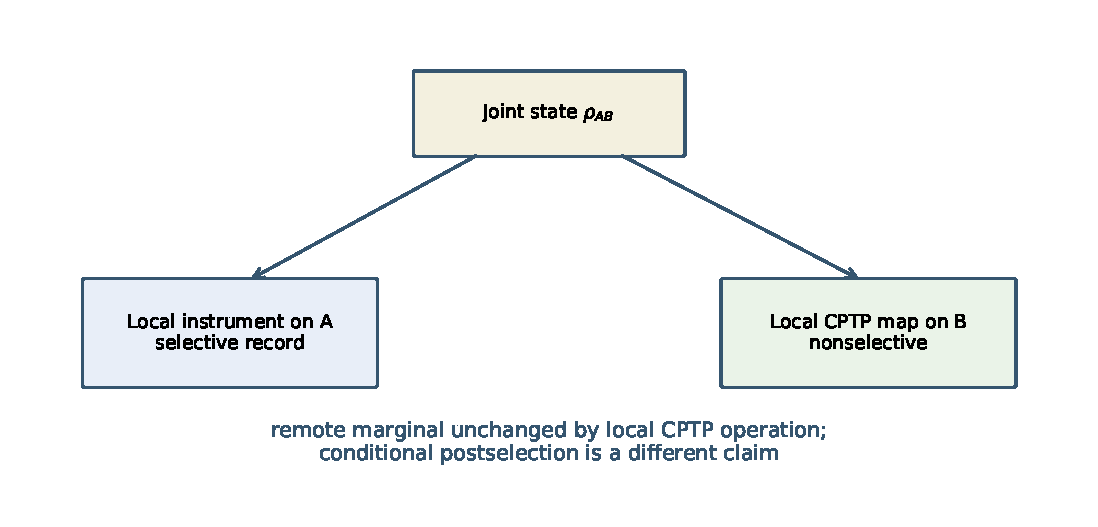
\includegraphics[width=0.90\linewidth]{../figures/fig_no_signalling_instrument.pdf}
\caption{Local deterministic operations preserve the remote marginal.
Selective outcomes update conditional states, but the nonselective sum and
classical outcome ledger prevent superluminal signalling.}
\label{fig:nosignal}
\end{figure}

Entanglement is therefore available once the tensor carrier is selected: it is
nonseparability of $\rho_{AB}$, not hidden classical correlation.  What remains
open is why the physical parent selects this tensor composition and its
occupied entangled states.  The no-signalling theorem is conditional on that
composition and cannot be used to derive it retrospectively.

\section{Measurement, decoherence and the classical limit}

\subsection{Quantum instrument}
A measurement terminal is represented by an instrument
$\{\mathcal I_a\}_a$, where each $\mathcal I_a$ is completely positive and
trace-non-increasing, and $\sum_a\mathcal I_a$ is CPTP.  Then
\begin{equation}
 p_a=\Tr\mathcal I_a(\rho),\qquad
 \rho_a=\mathcal I_a(\rho)/p_a.
\end{equation}
This is a consistent terminal record law.  It is not yet a proof of a physical
parent collapse.  The unconditioned state follows the deterministic channel;
the conditioned state records the selected outcome.

\subsection{Decoherence is not outcome selection}
For a preferred pointer algebra, a dephasing map removes off-diagonal phase
witnesses while preserving populations.  Markovian semigroups may be written
in Lindblad form \citep{Lindblad1976}.  Decoherence explains why interference
becomes inaccessible to a coarse observer and why stable records can behave
classically.  It does not select one realized outcome from the ensemble.

\subsection{Classical regime}
The classical limit used here requires all of the following:
\begin{enumerate}[label=(C\arabic*)]
\item suppression of phase-sensitive effects on the occupied record algebra;
\item redundant compatible records across accessible observer fragments;
\item a stable approximately commuting pointer algebra;
\item terminal resolutions coarse compared with the action-phase scale;
\item recovery errors below the declared record tolerance.
\end{enumerate}
The limit is therefore observer-relative but not arbitrary: it is constrained
by the occupied body relations and by independently testable record stability.

\section{Three distinct entropies}

Information loss in the descent defines a coarse-graining entropy, for example
the log measure of a stable fibre or the Shannon entropy of unresolved classes.
This quantity is not automatically the von Neumann entropy
\begin{equation}
 S_{\rm vN}(\rho)=-\Tr(\rho\log\rho),
\end{equation}
and neither is automatically thermodynamic entropy.  The identifications
require additional claims:
\begin{itemize}
\item coarse-graining entropy equals $S_{\rm vN}$ only when the quantum state
and its spectral probabilities are the sufficient observer record;
\item thermodynamic entropy requires a macroscopic state space, conserved
loads and an equilibrium or typicality argument;
\item entropy production requires irreversible effective dynamics or loss to
an inaccessible sector, not merely a many-to-one notation.
\end{itemize}
Recovery theory makes this distinction operational.  Exact sufficient
recovery can preserve relative entropy \citep{Petz1986}; correctable codes can
preserve the logical record even through a noisy physical carrier
\citep{KnillLaflamme1997}.  Hence information loss in one representation need
not be physical destruction of the occupied quantum information.

\section{Planck action scale}

Equation~\eqref{eq:schrodinger} shows what the Planck constant does in this
completion.  The parent packet supplies one action unit $U_A$ shared by phase
and clock descent.  Matching the terminal law to quantum mechanics identifies
\begin{equation}
 U_A=\hbar.
\end{equation}
This gives a structural interpretation: $\hbar$ is the action resolution that
converts source-owned phase transport into the observer's terminal clock and
energy units.  It is not proved to be a universal smallest parent action, and
the numerical SI value is not predicted.  A first-principles result would
require a source normalization tied independently to the base--seed action and
to operational SI standards.

\subsection{Downstream particle and RG handoff}

Technical Paper VII-C owns the scalar-15/type-II source preimage, its
class-relative mass/Planck ratio and the exact functional-RG evaluation law.
Paper VI does not rederive those results. It uses them only to delimit the
field-theory handoff: a selected particle branch may share the source action
unit while its occupation, component beta functions and SI calibration remain
separate physical obligations. The RG regulator is an analysis scheme, not
the observer-source quantizer \(Q_{OS}\) and not a quantum-readout mechanism.

\section{Quantum field theory recovery and frontier}

The finite carrier does not by itself yield QFT, but the theory hub already
contains a stronger conditional field packet than this paper previously
recorded.  Assume that the body descent supplies a globally hyperbolic metric
and a Green-hyperbolic free operator in the standard locally covariant
framework \citep{BrunettiFredenhagenVerch2003}.  Its
retarded-minus-advanced propagator has causal support, so spacelike-supported
observables commute.  On a stationary globally hyperbolic background, assume
a positive self-adjoint time-translation generator with no obstructing zero
modes and the regularity conditions required by the ground-state construction.
The resulting compatible pure quasifree covariance is then Hadamard
\citep{Radzikowski1996}.  Positivity of a generic time-dependent occupied
operator alone would not establish this conclusion.  The existing graph-normal
field/occupation block can then add a smooth coherent excitation without
changing the Hadamard singularity class.

For local interaction functionals, renormalized time-ordered products obeying
causal factorization generate relative $S$-matrices and spacelike-commuting
interacting local algebras order by order
\citep{BrunettiFredenhagen2000,HollandsWald2001}.  Thus the physical MVP
conditionally admits the standard architecture of perturbative QFT on curved
spacetime, including microcausality and the time-slice interpretation.  These
QFT results are imported conditional limits, not new Tau derivations.  The
Tau-specific question is whether one body-derived source packet supplies their
metric, state and local-interaction inputs without independent terminal
choices.  The paired bilocal control
shows why locality must remain an explicit source property: the same free
reduct admits nonlocal interactions.

This is not a nonperturbative construction and does not determine the
interaction density, couplings, renormalization conditions, spin-statistics,
gauge/BRST sector or Standard Model spectrum.  A generic time-dependent body
also need not select a unique vacuum.  Quantum stress and its stochastic
second cumulant can source a classical body-derived metric in the joint
functional, but a path integral over metrics, its gauge complex and a physical
inner product are not derived.  The current minimum branch is therefore
quantum matter/readout on a classical body-derived geometry, with stochastic
backreaction allowed; metric quantization remains undecided.

\section{Standard quantum recovery and Tau-specific discriminator}

The recovery result and the novelty claim must be kept separate.  Under the
frozen physical MVP, the following standard structures are recovered:
\begin{enumerate}[label=(R\arabic*)]
\item positive normalized density operators and POVMs;
\item the trace Born rule and coherent interference;
\item self-adjoint unitary transport with action unit $U_A=\hbar$;
\item tensor composition, singlet correlations and the Tsirelson value
$|S_{\rm CHSH}|=2\sqrt2$ on the selected two-qubit packet
\citep{Tsirelson1980};
\item invariance of a remote marginal under local nonselective CPTP maps;
\item free algebraic QFT and the perturbative causal construction under the
field assumptions above.
\end{enumerate}
These are necessary compatibility results, not Tau-specific deviations.

The proposed Tau discriminator concerns two quantities that would have to be
reconstructed by independent routes.  It is not yet an executable prediction,
because no audited carrier supplies the required independent action-side
observable.  For one predeclared occupied record pair define
\begin{equation}
 x_A:=\frac{\mathcal A_X^{PC}}{\mathcal A_*},
 \qquad
 x_Q:=d_{U,\mathrm{chord}}^2(\rho_0,\rho_1)
 =2\left(1-\sqrt{F(\rho_0,\rho_1)}\right).
 \label{eq:tau-action-uhlmann}
\end{equation}
The common-Gram completion predicts
\begin{equation}
 \boxed{x_A=x_Q.}
 \label{eq:tau-discriminator}
\end{equation}
Standard quantum mechanics determines $x_Q$ from state tomography but has no
independent morphological action variable $x_A$ and therefore does not imply
Eq.~\eqref{eq:tau-discriminator}.  This cross-domain identity, rather than a
modification of the Born rule, is the primary conditional Tau discriminator.

The prediction remains quantitative under certified approximate recovery.
If a record map $\mathcal C$ has a recovery $\mathcal R$ satisfying
$\sup_\rho\|\mathcal R\mathcal C(\rho)-\rho\|_1\le\eta$ on the frozen state
family, contractivity and the Bures triangle inequality give
\begin{equation}
 0\le x_A-x_Q^{\rm out}
 \le x_A-
 \left[\max\left\{0,\sqrt{x_A}-2\sqrt\eta\right\}\right]^2.
 \label{eq:approx-tau-discriminator}
\end{equation}
Thus recovery uncertainty broadens the equality into a precomputable interval;
it is not an adjustable fit.

Writing $x_A=\epsilon_O^2$, the common-Gram identity gives the Bures angle
$D_B=2\arcsin(\epsilon_O/2)$.  For a constant energy spread under a declared
self-adjoint unitary protocol, the standard quantum speed limit then yields
\begin{equation}
 \delta t_{\min,O}\ge
 \frac{2\hbar}{\Delta H}\arcsin\frac{\epsilon_O}{2}
 \ge\frac{\hbar\epsilon_O}{\Delta H}.
 \label{eq:qor-discriminator}
\end{equation}
The inverse-energy law and Bures speed limit are standard
\citep{MandelstamTamm1945,AnandanAharonov1990}.  Tau Core predicts that their
distance input is fixed by an independently measured morphological action
separation.  A timing violation can reject the occupied completion only after
Eq.~\eqref{eq:tau-discriminator}, record hold, recovery quality and $\Delta H$
have been certified independently.

Define the preregistered residual
\begin{equation}
 \Delta_{AQ}:=x_Q^{\rm out}-x_A.
\end{equation}
Exact recovery predicts $\Delta_{AQ}=0$; approximate recovery predicts the
one-sided interval in Eq.~\eqref{eq:approx-tau-discriminator}.  A statistically
significant value outside that interval falsifies the common-Gram physical
MVP for the tested carrier.  Passing it supports the shared-source identity
but does not uniquely establish Tau Core, because another theory could impose
the same relation.  The model currently predicts no universal numerical
$\epsilon_O$ or laboratory effect size; those require identification of a
physical carrier and independent action reconstruction.

\section{Public-data audit}

We next ask how far Eq.~\eqref{eq:tau-discriminator} can be tested without a
new laboratory protocol.  Two public same-carrier datasets already provide
nontrivial controls.  Tan et al. measured the quantum metric of one
superconducting qubit by both sudden quench and weak periodic drive
\citep{Tan2019QGT}.  Extraction from the public vector figures gives 17
matched $g_{\phi\phi}$ points with Pearson correlation $0.9892$, MAE
$0.01952$ and RMSE $0.02222$; nine nearly constant $g_{\theta\theta}$ points
give MAE $0.00959$.  The observed cross-protocol offsets are comparable to
published decoherence, finite-time and control scales, so they cannot be
identified as a Tau gain.

Yu et al. measured metric components and Berry curvature on an NV-centre
carrier using distinct parametric modulations \citep{Yu2019QGT}.  On the seven
non-boundary matched coordinates, the pure-qubit identity
\begin{equation}
 |F_{\theta\phi}|=
 2\sqrt{g_{\theta\theta}g_{\phi\phi}-g_{\theta\phi}^2}
\end{equation}
has Pearson correlation $0.9933$, MAE $0.01545$ and RMSE $0.01577$ in the
public vector-figure extraction.  This independently replicates a
cross-readout local quantum geometry on a second platform.

These positive results support the standard quantum-geometric recovery and a
local same-carrier connector proxy.  They do \emph{not} test the finite Tau
identity.  Every reconstructed axis is a standard quantum-geometric terminal;
none is an independently measured once-counted morphological action
$\mathcal A_X^{PC}$.  The public figures also do not provide a certified
finite Uhlmann endpoint pair with the required recovery ledger.  Therefore
current public data determine neither $x_A$ nor $\Delta_{AQ}$.  This is a
finite identifiability no-go, rather than a null Tau result: the datasets
validate part of the standard-recovery side but cannot confirm or falsify
Eq.~\eqref{eq:tau-discriminator}.  The frozen points, provenance manifest and
recalculation script are included in the reproducibility package.

\subsection{Compact audit verdict}

A frozen public-carrier census applied five hard gates: same carrier, an
$x_Q$-capable endpoint distance, an action-like observable, an independently
once-counted $x_A$, and an uncertainty/recovery ledger.  None of the audited
candidates passes the independent-$x_A$ gate.  The strongest standard controls
confirm ordinary quantum geometry and speed-limit behavior, but they do not
supply the cross-domain observable required by
Eq.~\eqref{eq:tau-discriminator}.  The result is therefore an identifiability
no-go, not a negative Tau detection.

\begin{table}[ht]
\centering
\small
\caption{Compact public-carrier verdict.  ``Partial'' denotes a model-dependent
or same-pipeline proxy.  The full candidate-by-candidate ledger is preserved in
the technical supplement.}
\label{tab:public-census}
\begin{tabularx}{\textwidth}{@{}Xcccc@{}}
\toprule
Carrier class & same carrier & $x_Q$ & independent $x_A$ & recovery/errors\\
\midrule
QGT and tomography platforms & yes & yes & no & partial\\
Quantum-speed-limit platforms & yes & yes & no & yes/partial\\
Work, calorimetry and source-port platforms & yes & partial & no & partial\\
Optical path-integral data & yes & partial & no & partial\\
\bottomrule
\end{tabularx}
\end{table}

The strongest QOR control, the trapped-atom data of Ness et al.\
\citep{Ness2021QSL}, is consistent with the standard speed limit: no one-sided
violation among 53 public points exceeds $1.96\sigma$ (maximum
$1.4465\sigma$).  The Wen optical reconstruction reproduces the phase control
and reveals a standard kernel-morphology amplitude dependence, but the
source-frozen Tau curvature candidate is null and the optical action is not an
independent Tau body action.  These results validate parts of the standard
recovery pipeline without evaluating $x_A=x_Q$.

There is also a structural no-go.  Tomography, QGT and fidelity are circular as
$x_A$ estimators; band curvature and state-space QGT are independent in a
finite two-band countermodel; energy and fidelity susceptibilities are
different spectral moments; and equal local stiffness does not determine a
finite Uhlmann chord or loop holonomy.  Consequently the minimum admissible
reopening packet is
\begin{equation}
 \boxed{\{K_A,\ C_q,\ \nabla^C,\ A_*,\
          \text{withheld endpoints, loops and recovery ledger}\}}.
 \label{eq:minimal-blind-packet}
\end{equation}
The body-side stiffness and its action unit must be frozen before the quantum
endpoints are examined.

The internal finite audits sharpen but do not remove this boundary.  The
inherited CHDF quotient supplies a positive body-side action candidate, and
exact recovery selects the identity member inside a bounded depolarizing
connector family.  Generic CPTP structure does not select that member, and
ordinary thermodynamic work is not universally proportional to the Bures
chord.  Thus the remaining physical question is occupation of one common
source packet, not another fit of terminal data.

The complete candidate census, all finite countermodels, the alternative
source-port survey, Wen path reconstruction, readiness scores and detailed
claim boundaries are retained in the separately compiled
\emph{Public-Data and Source-Port Audit for the Tau Core Quantum Terminal}.
The scripts and frozen data used by both documents remain in this repository.

\section{Finite decision protocol}

The theory does not need unlimited data collection to test this packet.  It
needs one source-frozen carrier family on which the following finite gates are
independently reconstructed:
\begin{enumerate}[label=(F\arabic*)]
\item a stable observer partition and ordered record transitions;
\item a positive response metric $g$ and phase curvature $\omega$;
\item the lock residual
$r_J=\| (g^{-1}\omega)^2+\kappa^2I\|$;
\item a phase-sensitive interference witness excluded by the classical
same-quotient control;
\item a normalized positive effect ledger testing Eq.~\eqref{eq:born};
\item a compositional no-signalling test with selective and nonselective
controls;
\item a recovery/dephasing control separating transport loss from outcome
statistics.
\item independent same-carrier reconstructions of $x_A$ and $x_Q$, with the
recovery tolerance $\eta$ frozen before evaluating
Eq.~\eqref{eq:tau-discriminator};
\item only after that identity passes, an independent $\Delta H$ and timing
test of Eq.~\eqref{eq:qor-discriminator}.
\end{enumerate}

The branch is weakened if $r_J$ remains nonzero beyond uncertainty, if the
phase witness vanishes while the proposed quantum packet is occupied, if
probabilities require context-dependent gains, or if a local deterministic
operation changes a remote marginal.  Passing these tests establishes the
finite terminal packet, not its unique parent origin.

\section{Parent-realization theorem and exact boundary}

Let $\mathfrak P_Q$ denote the complete packet consisting of the positive
metric, nondegenerate phase form, compatible complex structure, common action
unit, separating positive effects, tensor composition and exact recovery on
the occupied logical algebra. The present base--seed reduct does not entail
$\mathfrak P_Q$. Keep the stabilized body, occupied P3 algebra, normalized
positive states and upstream source data fixed, and consider
\begin{equation}
 \mathcal C_\gamma(\rho)
 =\gamma\rho+(1-\gamma)I/2,
 \qquad 0\leq\gamma\leq1.
 \label{eq:joint-packet-counterfamily}
\end{equation}
Both $\gamma=1$ and $\gamma=1/2$ are CPTP descents of the same upstream
packet. Orthogonal-state trace distance becomes $\gamma$. If a CPTP left
inverse existed on the full logical algebra, contractivity of that inverse
would require $1\leq\gamma$. Hence $\gamma=1$ realizes exact recovery and
the bounded A8b connector, whereas $\gamma=1/2$ does not. The aligned and
irreducible occurrence transports provide an independent equal-reduct pair
with tensor-orbit ranks three and five. Therefore
\begin{equation}
 B_\tau^{\rm phys}+s_U
 \not\Longrightarrow \mathfrak P_Q
 \label{eq:joint-packet-nonentailment}
\end{equation}
under the current axioms.

There is nevertheless an exact sufficient source criterion. Call one
occupied once-counted parent representation source-faithful and protected
when it is simultaneously: (i) action-isometric with the common
Hilbert--Schmidt/Uhlmann unit; (ii) metric--symplectic; (iii) separating on
the occupied P3 operator system; (iv) monoidal through two faithful commuting
$M_2(\mathbb C)$ factors; and (v) exactly recoverable on the designated
logical algebra, with loss confined to its sourced realization complement.
For such an $\mathrm{SFPR}_Q$, the preceding theorems give respectively the
complex structure, GNS/Born pairing, complete effect atlas, tensor locality,
exact A8b member and inherited action unit. Thus
\begin{equation}
 \mathrm{SFPR}_Q\Longrightarrow\mathfrak P_Q.
 \label{eq:sfpr-sufficient}
\end{equation}
This is a representation theorem, not an existence theorem. The remaining
remaining unrestricted input is physical base--seed occupation of one
$\mathrm{SFPR}_Q$; declaring it would close the MVP conditionally, while
deriving it requires a stronger parent action or independent physical
evidence.

The recovery component has a sharper physical selector. Let
$\mathcal C_O^c$ be a complementary channel of observer descent. If, on an
isolated occupied logical algebra,
\begin{equation}
 \mathcal C_O^c(\rho_L)=\tau_G
 \quad\text{for every }\rho_L,
 \label{eq:logical-nonleakage}
\end{equation}
then the inaccessible realization complement contains no logical-state
information. The finite-dimensional information--disturbance/correctability
criterion \citep{KnillLaflamme1997} implies
a CPTP left inverse of $\mathcal C_O$ on the complete logical algebra. At the
same minimal input and output dimension the channel is unitary conjugation.
This condition is stronger than stable classical recording: complete
dephasing preserves the trace distance of $|0\rangle,|1\rangle$ but maps the
orthogonal phase pair $|+\rangle,|-\rangle$ to the same state.

A parent-side sufficient realization of Eq.~\eqref{eq:logical-nonleakage} is
a source-frozen isolated split $T M_{\rm occ}=L\oplus G$ satisfying
\begin{equation}
 P_LH_{\rm parent}P_G=0,\qquad
 \ell_{\rm parent}=\ell_L\oplus\ell_G,qquad
 U_{\rm parent}=U_L\otimes U_G,qquad
 \rho_{LG}=\rho_L\otimes\tau_G.
 \label{eq:morphological-isolation}
\end{equation}
Thus morphological isolation means absence of a mixed source incidence able
to export logical distinguishability into $G$, not absence of the surrounding
body. The observed unitary limit of isolated quantum systems requires this
law operationally. It is therefore a 4D-constrained isolated-scope selector,
not yet a first-principles consequence of the current base--seed action.
Turning on the mixed block gives the approximate-recovery regime rather than
a contradiction.

\subsection{Disjoint-source valuation and the isolation theorem}

This source-locality proposal should not be confused with standard cluster
decomposition or with algebraic-QFT locality.  Those are terminal statements
about correlations or commuting observable algebras.  The valuation below is
a stronger parent-side composition axiom for disconnected occupied source
incidences; the paper tests its consequences without claiming that standard
locality selects it.

The block-zero condition in Eq.~\eqref{eq:morphological-isolation} follows
from one finite parent composition law. Let the occupied source hypergraph
split into disconnected components and require the once-counted parent action
to be a normalized disjoint-union valuation,
\begin{equation}
 \mathcal A(\varnothing)=0,\qquad
 \mathcal A(X\sqcup Y)=\mathcal A(X)+\mathcal A(Y)
 \label{eq:disjoint-source-valuation}
\end{equation}
whenever no occupied primitive source incidence meets both $X$ and $Y$.
Induction on the finite connected-component decomposition gives
\begin{equation}
 \mathcal A(H_{\rm occ})=\sum_c\mathcal A(H_c).
 \label{eq:component-action-sum}
\end{equation}
Twice differentiating Eq.~\eqref{eq:component-action-sum} yields
\begin{equation}
 P_cH_{\rm parent}P_d=0\qquad(c\neq d).
 \label{eq:component-hessian-zero}
\end{equation}
Equations~\eqref{eq:disjoint-source-valuation}--\eqref{eq:component-hessian-zero}
therefore prove only the action and Hessian parts of morphological isolation.
Exact logical recovery additionally requires the source load, generator and
occupied state to factor as stated explicitly in
Eq.~\eqref{eq:morphological-isolation}, or an independent proof of the
logical non-leakage condition~\eqref{eq:logical-nonleakage}.  A vanishing
mixed Hessian alone does not exclude higher-order, global-constraint or
initial-correlation leakage.

The valuation is not implied by once-counting, positivity, source freeze and
internal component symmetry alone. A positive parent Hessian may contain
\begin{equation}
 \epsilon\,
 \langle z_L,\mathbf 1\rangle
 \langle z_G,\mathbf 1\rangle,
 \qquad \epsilon\neq0,
 \label{eq:hidden-cross-counterterm}
\end{equation}
while preserving the two internal permutation symmetries. Equation
\eqref{eq:hidden-cross-counterterm} gives
$P_LH_{\rm parent}P_G\neq0$ and violates
Eq.~\eqref{eq:disjoint-source-valuation}. The valuation is therefore a real
composition law, not a restatement of the weaker source packet.

If a physical hyperedge crosses the $L|G$ partition, its second variation may
generate precisely such a mixed block. Logical information can then enter
$G$, allowing entanglement, local decoherence and nonexact recovery while the
joint parent state remains represented. Exact protection is consequently an
isolated-scope theorem, not a universal ban on interaction.

\subsection{Operational-to-parent two-jet lifting theorem and no-go}

The finite valuation defect
$\mathcal A(X\sqcup Y)-\mathcal A(X)-\mathcal A(Y)$ is a scalar and cannot be
acted on by a terminal Jacobian.  The operationally accessible local object is
instead its mixed second variation.  For source variations
$u\in E_X$ and $v\in E_Y$, define
\begin{equation}
 N_{\mathcal A}^{X|Y}(u,v)
 :=\left.\frac{\partial^2}{\partial s\,\partial t}
 \mathcal A\bigl(X(su)\sqcup Y(tv)\bigr)\right|_{s=t=0}
 \in E_{\rm cross}:=\operatorname{Bil}(E_X,E_Y;\mathbb R).
 \label{eq:parent-two-jet-defect}
\end{equation}
Let
$\mathfrak D_{\rm prim}^{(2)}:E_{\rm cross}\to E_{\rm term}^{(2)}$
be the stacked, source-frozen second-jet descent of all declared primitive
physical readouts.  This typed map sends a parent mixed bilinear response to
the corresponding family of terminal mixed responses.

\begin{proposition}[Joint two-jet faithfulness]
Suppose operationally isolated preparations have vanishing mixed terminal
responses,
\begin{equation}
 \mathfrak D_{\rm prim}^{(2)}N_{\mathcal A}^{X|Y}=0,
\end{equation}
for every admissible pair, and suppose
\begin{equation}
 \ker\mathfrak D_{\rm prim}^{(2)}\cap E_{\rm cross}=\{0\}.
 \label{eq:cross-defect-faithfulness}
\end{equation}
Then $N_{\mathcal A}^{X|Y}=0$, equivalently
$P_XH_{\rm parent}P_Y=0$, on that occupied scope.
\end{proposition}

\begin{proof}
The operational premise places $N_{\mathcal A}^{X|Y}$ in
$\ker\mathfrak D_{\rm prim}^{(2)}$, while
Eq.~\eqref{eq:parent-two-jet-defect} places it in $E_{\rm cross}$.
Equation~\eqref{eq:cross-defect-faithfulness} makes this intersection trivial.
\end{proof}

This proposition lifts only the local mixed two-jet.  It does not recover the
finite valuation law~\eqref{eq:disjoint-source-valuation}: that stronger
statement requires all mixed finite-response jets to vanish, or an independent
global composition axiom.  Nor does the proposition alone imply exact
recovery, which still requires the remaining factors in
Eq.~\eqref{eq:morphological-isolation}.

The faithfulness premise is necessary for \emph{universal identifiability over
the admitted cross-defect class}.  Add to a positive valuation Hessian a small
positive-preserving cross form $N$ such that
\begin{equation}
 P_LNP_G\neq0,\qquad \mathfrak D_{\rm prim}^{(2)}N=0.
 \label{eq:equal-readout-hidden-parent}
\end{equation}
The original and modified parents have identical declared primitive two-jet
reducts, while only the first has a zero mixed Hessian.  Thus no inference
valid for the full admitted defect class can establish parent two-jet
isolation while a common cross-defect null direction survives.  A narrower
physical model may exclude the counterform by an additional source law, so
faithfulness is not asserted as a logically necessary axiom of every possible
completion.

The present series does not yet establish
Eq.~\eqref{eq:cross-defect-faithfulness}. A global physical
$\mathfrak D_{\rm prim}^{(2)}$ cannot yet be formed on one frozen domain because full
electric/magnetic/radiative gravity, photon and gauge occupation,
non-Abelian/chiral matter, interacting multi-system QFT and their common
calibration are not all completed. The local six-dimensional Green packet is
complete on its own descriptor, but that local rank statement is not global
primitive-readout completeness. Thus the exact status is
\begin{equation}
 \begin{gathered}
 \text{joint two-jet faithfulness}
 \Longrightarrow
 \text{zero parent mixed Hessian},\\
 \text{zero parent mixed Hessian}
 +\text{ global factorization data}
 \Longrightarrow \text{protection},
 \end{gathered}
 \label{eq:valuation-proof-chain}
\end{equation}
with the first premise physically open and an equal-readout countermodel
excluding a stronger universal inference from the current reduct.  In
particular, the absence of a completed global terminal stack establishes
non-demonstrability, not a theorem that the physical kernel is nonzero.

The possibility-space intuition requires one further distinction. Let
$C_x^+$ be the forward cone selected by the body order and $K_x>0$ the local
body Hessian. If the local admissibility law is reversal symmetric, then
$v\mapsto-v$ is an isometry between the forward and backward quadratic
acceptance bodies. Orientation and stiffness alone therefore cannot enlarge
the future. Let $R_-$ and $R_+$ instead denote the source-owned restriction
maps imposed on backward and forward compatible extensions. Their fibres are
\begin{equation}
 F_x^- = \ker R_-,\qquad F_x^+=\ker R_+.
 \label{eq:future-extension-fibres}
\end{equation}
A larger future possibility space means a larger dimension or inherited
Hessian volume of $F_x^+$, as can occur when seed and current-body data fix
backward compatibility more strongly than forward completion.

This asymmetry becomes exact when backward extension must also reproduce the
observer's already stable records. Let $R_{\rm rec}$ be the corresponding
record-agreement map on the current cut and set
\begin{equation}
 R_-=(R_+,R_{\rm rec}).
 \label{eq:record-conditioned-restriction}
\end{equation}
Then
\begin{equation}
 F_x^-=ker R_+\cap\ker R_{\rm rec}\subseteq F_x^+,
 \qquad
 \dim F_x^+-\dim F_x^-
 =\operatorname{rank}\!\left(R_{\rm rec}|_{F_x^+}\right).
 \label{eq:future-fluidity-rank-theorem}
\end{equation}
The second identity is rank--nullity applied to the restricted record map.
Consequently the future fibre is strictly larger exactly when a stable record
constraint removes at least one otherwise future-compatible direction. At
fixed resolution $\epsilon$, $r$ independent removed directions can increase
the operational number of resolved future cells relative to past cells by a
factor scaling as $\epsilon^{-r}$ on a normalized bounded chart. This cell
count, rather than a comparison of volumes in different dimensions, is the
precise sense in which the future can be much more ``fluid.''

No stored parent history is used: $R_{\rm rec}$ is a simultaneous stability
condition in the observer's current readout quotient. Nor does the observer
access actual future outcomes. Equation~\eqref{eq:future-fluidity-rank-theorem}
establishes excess compatible directions, not their quantum coherence; the
phase form and future--ROOT bridge remain necessary for that promotion.

The word ``larger'' does not mean unbounded. The admissible local future body
is
\begin{equation}
 \mathcal E_x^+(\Lambda)
 =F_x^+\cap C_x^+\cap\mathcal D_M
  \cap\{v:g_+(v,v)\leq\Lambda\},
 \label{eq:bounded-future-possibility-body}
\end{equation}
where $\mathcal D_M$ contains the remaining morphology constraints. If
$F_x^+$ is finite dimensional, $g_+>0$, $\Lambda<\infty$ and the causal and
morphology constraints are closed, Eq.~\eqref{eq:bounded-future-possibility-body}
is compact and has finite Hessian volume. A finite observer resolution then
produces only finitely many stable readout cells. The future is more fluid
only relative to the record-constrained past; the morphological body still
sets its directions, stiffness, boundary and accessible resolution.

The available concrete body quotient also gives an exact dimensional
boundary.  The CHDF leaf Hessian is positive on one radial and two tangent
directions, hence has real rank three.  If that leaf alone were identified
with $F_x^+$, every linear bridge to the real rank-four ROOT qubit would have
rank at most three; an antisymmetric phase form on the leaf has even rank at
most two.  Thus the CHDF-leaf-only identification cannot realize the full
ROOT carrier.  This is not a no-go for the enriched body: the P3/ROOT packet
already supplies the conditional rank-four target, but no source-frozen
body-first matrix $R_+$ is currently available on that same domain.  The
numerical rank of the mixed future--ROOT block is consequently undefined,
not zero.  The next finite construction is an enriched body/P3 restriction
retaining a four-real-dimensional non-gauge, metric-visible sector before
the ROOT terminal is applied.

The inclusion $i_+:F_x^+\hookrightarrow T_xM_\tau$ induces
\begin{equation}
 g_+=i_+^*K_x>0.
 \label{eq:future-fibre-metric}
\end{equation}
This is a classical possibility geometry. A symmetric Hessian cannot itself
produce phase. If the same source supplies a quotient-basic curvature
$\omega_+$ with
\begin{equation}
 (g_+^{-1}\omega_+)^2=-\kappa^2I,
 \label{eq:future-phase-lock}
\end{equation}
then $J_+=g_+^{-1}\omega_+/\kappa$ gives the complex carrier and the existing
coherent positive-effect theorems apply. The observer accesses a current
descriptor of the compatible extension fibre, not an already realized future
outcome. Operational future-blindness and no-signalling are therefore
preserved. Physical realization of $R_+$, its rank advantage and the common
source of $\omega_+$ remain open.

The last open phrase can be sharpened by using the variational boundary
structure of one parent action rather than postulating an unrelated phase
law. Suppose an ordered differentiable parent action has first variation
\begin{equation}
 \delta\mathcal A_M
 =\langle E(M),\delta M\rangle
  +\int_{\Sigma_O}\theta_M(\delta M),
 \label{eq:parent-boundary-variation}
\end{equation}
where $\Sigma_O$ is the current observer cut. On compatible linearized future
solutions, the bulk second variation induces the Jacobi metric $g_+$, while
the antisymmetrized boundary variation induces
\begin{equation}
 \omega_+(\delta_1,\delta_2)
 =\delta_1\theta_M(\delta_2)-\delta_2\theta_M(\delta_1).
 \label{eq:future-presymplectic-form}
\end{equation}
Thus metric and phase have one once-counted variational owner. After removing
the gauge/null kernel, assume $g_+>0$ and nondegenerate $\omega_+$. With
$A=g_+^{-1}\omega_+$, polar decomposition gives
\begin{equation}
 J_+=A(-A^2)^{-1/2},\qquad J_+^2=-I.
 \label{eq:future-polar-complex-structure}
\end{equation}
This conditionally derives the complex carrier without an independent phase
gain. It does not imply the stronger scalar lock
$A^2=-\kappa^2I$: that requires all polar mode scales to coincide. The finite
certificate with $g_+=\operatorname{diag}(1,1,2,2)$ and two equal canonical
phase blocks has a valid polar complex structure but mode scales
$(1,1,1/2,1/2)$. It is therefore an explicit counterexample to deriving one
universal action unit from common variational ownership alone. Physical
occupation, quotient descent and the equal-mode-scale law remain open.

The equal-mode-scale condition itself has a finite representation-theoretic
closure. Let a parent symmetry group $G$ act irreducibly on the occupied real
future fibre and preserve both $g_+$ and $\omega_+$. Then
$A=g_+^{-1}\omega_+$ commutes with $G$, and so does the positive self-adjoint
polar operator $|A|=(-A^2)^{1/2}$. Every eigenspace of $|A|$ is $G$-invariant.
Irreducibility therefore forces
\begin{equation}
 |A|=\kappa I,\qquad A^2=-\kappa^2I.
 \label{eq:irreducible-polar-scale-lock}
\end{equation}
This is the required scalar lock, not an additional fitted gain. A real
four-dimensional quaternionic certificate has a one-dimensional symmetric
commutant and zero lock residual. By contrast, a reducible sum of two phase
planes retains scales $1$ and $1/2$. Thus irreducibility is essential. The
current base--seed law has not yet been shown to occupy this irreducible
future-fibre orbit, and Eq.~\eqref{eq:irreducible-polar-scale-lock} fixes only
relative mode scales, not the absolute value or SI calibration of $\kappa$.

No new irreducible carrier is required for this step. The occupied logical
ROOT qubit is a complex two-dimensional, hence real four-dimensional,
irreducible $SU(2)$ module. Let
\begin{equation}
 C_{FQ}:F_x^+\longrightarrow \mathcal H_{\rm ROOT}^{\mathbb R}
 \label{eq:future-root-bridge}
\end{equation}
be a source-owned bijective intertwiner preserving the metric and phase
forms. Pulling the ROOT action back through $C_{FQ}$ makes $F_x^+$
irreducible, so Eq.~\eqref{eq:irreducible-polar-scale-lock} follows. The
finite realified Pauli certificate has bridge rank four, zero intertwining
residual and a one-dimensional symmetric commutant.

Equation~\eqref{eq:future-root-bridge} is not selected by the current reduct.
Keeping the stabilized body and complete internal ROOT packet fixed admits
both $C_{FQ}=0$ and a full-rank equivariant $C_{FQ}$. Thus the bridge theorem
reduces physical occupation to one typed source incidence but does not derive
that incidence from the present base--seed law.

The source of $C_{FQ}$ can be localized further. Decompose the boundary
second variation of Eq.~\eqref{eq:parent-boundary-variation} into future and
ROOT blocks,
\begin{equation}
 \omega_{\partial M}=
 \begin{pmatrix}
  \omega_F & \beta_{FQ}\\
  -\beta_{FQ}^{T} & \omega_Q
 \end{pmatrix}.
 \label{eq:mixed-future-root-boundary-form}
\end{equation}
If $F_x^+$ and $\mathcal H_{\rm ROOT}^{\mathbb R}$ are equivalent
irreducible parent modules and $\beta_{FQ}$ is a nonzero equivariant
intertwiner, then its kernel and image are invariant. Irreducibility forces a
zero kernel and full image, so $\beta_{FQ}$ itself supplies a full-rank
$C_{FQ}$. Separate bijectivity is not an independent assumption.

The diagonal restrictions $\omega_F$ and $\omega_Q$ do not activate this
block. A finite antisymmetric family with the same two diagonal phase forms
admits both $\beta_{FQ}=0$ and $\beta_{FQ}=\lambda I$; for
$0<|\lambda|<1$ the latter joint form is nondegenerate and its bridge has rank
four. Hence common variational ownership alone still does not force the mixed
incidence. This block is distinct from the forbidden logical--environment
mixing in Eq.~\eqref{eq:morphological-isolation}: $\beta_{FQ}$ loads the
protected logical carrier from the body possibility fibre, while morphological
isolation prevents that logical information from leaking into the inaccessible
realization complement.

The previously derived BRAC term does not by itself supply this boundary
block. Its morphology-dependent potential is zeroth order, so it has a
generically nonzero mixed bulk Hessian on an occupied field but contributes no
independent covariant symplectic potential. The required source instead occurs
in the covariant kinetic term of the selected joint completion
(JCSEL, BRDC and EBRP). On an observer cut its canonical momentum is
\begin{equation}
 \pi_\Phi=Z_\Phi\sqrt h\,n^\mu\partial_\mu\Phi.
 \label{eq:body-dependent-field-momentum}
\end{equation}
For a future body variation $\delta_F$ and field variation $\delta\Phi$, the
mixed boundary coefficient contains
\begin{equation}
 \beta_{FQ}(\delta_F,\delta\Phi)
 \supset \delta_F\!\left(Z_\Phi\sqrt h\,n^\mu\right)
 \partial_\mu\Phi\,\delta\Phi.
 \label{eq:kinetic-future-root-activation}
\end{equation}
SBTCL595's nonneutral EBRP branch supplies a nonzero occupied
positive-frequency field momentum. Hence every non-gauge future mode that
changes the densitized normal kinetic metric makes
Eq.~\eqref{eq:kinetic-future-root-activation} nonzero. Covariance makes the
block equivariant; on the equivalent irreducible future/ROOT sector the
preceding Schur argument promotes it to the full bridge.

This proves activation inside the selected covariant working completion. It
does not prove that the physical base--seed parent selects JCSEL--BRDC--EBRP,
that the realized body is nonneutral, or that every future-fibre direction is
metric-visible. The unrestricted physical statement therefore remains conditional,
while the internal completion question is closed.

\section{What is proved and what remains open}

\begingroup
\small
\sloppy
\begin{longtable}{@{}>{\raggedright\arraybackslash}p{0.23\linewidth}>{\raggedright\arraybackslash}p{0.50\linewidth}>{\raggedright\arraybackslash}p{0.18\linewidth}@{}}
\caption{Claim ledger.  ``Conditional theorem'' means mathematically derived
from the explicitly frozen packet, not established as an unrestricted
parent-law realization with physical occupation.}
\label{tab:ledger}\\
\toprule
Claim & Status and condition & Class \\
\midrule
\endfirsthead
\multicolumn{3}{c}{\small\itshape Claim ledger (continued)}\\
\toprule
Claim & Status and condition & Class \\
\midrule
\endhead
\midrule
\multicolumn{3}{r}{\small\itshape Continued on next page}\\
\endfoot
\bottomrule
\endlastfoot
Loss alone implies quantum mechanics & False; classical and quantum
completions share one finite quotient & No-go theorem \\
Complex carrier & Follows from positive $g$, nondegenerate $\omega$ and
$A^2=-\kappa^2I$ & Conditional theorem \\
Unitary transport & Follows from Paper-V time, one action unit and commuting
self-adjoint $K$ & Conditional theorem \\
Born and interference & Follows from positive trace effects and coherent
composition & Conditional theorem \\
No-signalling & Follows for local CPTP maps after tensor composition is fixed
& Conditional theorem \\
Measurement & Quantum instruments are consistent; physical single-outcome
selection is not derived & Open physics \\
Classical limit & Decohered commuting records give a controlled effective
limit; not a fundamental collapse & Conditional limit \\
Planck scale & $U_A=\hbar$ by standard-limit calibration; SI value not derived
& Identification \\
Downstream scalar-15 scale and interacting RG & owned by Technical Paper
VII-C; imported only as a field-theory boundary & not part of the quantum
terminal derivation \\
Current reduct selects the packet & False:
Eq.~\eqref{eq:joint-packet-counterfamily} gives an equal-upstream-reduct
counterfamily & Exact non-entailment theorem \\
Joint source criterion & One occupied source-faithful protected
representation implies the complete packet by Eq.~\eqref{eq:sfpr-sufficient};
its physical occupation is open & Conditional representation theorem \\
Isolation selector & Logical non-leakage in
Eq.~\eqref{eq:logical-nonleakage} forces exact recovery; the factorized parent
law in Eq.~\eqref{eq:morphological-isolation} is sufficient but not yet
derived from the base--seed action & Theorem plus physical-MVP selector \\
Disjoint-source valuation & Exact finite additivity forces a block-diagonal
Hessian, but the Hessian statement alone does not force global dynamics,
state factorization or recovery & Conditional composition theorem \\
Operational parent lift & Jointly faithful typed second-jet descent lifts
vanishing terminal mixed responses to a zero parent mixed Hessian; it does not
derive finite valuation or recovery by itself, and global faithfulness is not
yet demonstrable & Conditional local theorem plus identifiability no-go \\
Future-extension carrier & Boundary-fibre asymmetry can enlarge the forward
possibility space and the restricted Hessian supplies its metric; phase lock
and physical fibre selection remain conditional & Theorem/no-go plus
conditional completion \\
Record-conditioned fluidity & Stable backward record agreement gives
$F_x^-\subseteq F_x^+$ with dimension gap equal to the restricted record rank;
coherence of the excess directions is not automatic & Exact rank theorem \\
Bounded future body & Positive restricted Hessian, finite action cutoff and
closed body/causal constraints make the admissible future compact with finite
observer-resolved cell count & Conditional compactness theorem \\
Common-action phase source & Bulk and boundary variations of one parent action
conditionally supply $g_+$ and $\omega_+$; polar decomposition gives $J_+$,
but equal polar scales and one universal action unit do not follow &
Conditional theorem plus finite no-go \\
Irreducible mode-scale lock & A common parent symmetry preserving $g_+$ and
$\omega_+$ forces $|g_+^{-1}\omega_+|=\kappa I$ on an irreducible occupied
future fibre; physical orbit occupation and absolute calibration remain open
& Conditional Schur-rigidity theorem \\
Future--ROOT bridge & A bijective source-owned metric--phase intertwiner to the
logical ROOT qubit transfers its real irreducibility and closes the relative
scale lock; zero/full-rank equal-reduct completions prove current nonselection
& Conditional bridge theorem plus exact non-entailment \\
Mixed boundary source & A nonzero equivariant future--ROOT boundary block is
automatically full rank between the equivalent irreducible carriers; identical
diagonal packets admit zero/nonzero blocks, so physical activation is open &
Conditional Schur theorem plus exact counterfamily \\
Kinetic activation & BRAC bulk mixing is the wrong type, but the selected
JCSEL--BRDC--EBRP kinetic momentum gives $\delta_F\pi_\Phi\neq0$ for occupied
non-null metric-visible future modes; unrestricted completion realization remains
open & Conditional physical-completion theorem \\
Single-system common source & Derived inside the enriched MVP plus adopted
P3 handoff; unchanged-parent realization remains open & Conditional source
theorem \\
P3 handoff selector & Separating records with one common scalar quadratic
action force the operator-square and graph-normal law; physical occupation
remains open & Conditional source theorem \\
P3 record rank & Primitive and binary families have kernels $56$ and $35$;
grade-$\leq3$ closure has rank $64$; physical ternary occupation remains open
& Exact finite rank theorem \\
Spectral record atlas & Canonical binary effects of all grade-$\leq3$ words
are separating; Frobenius pointer copying alone has rank eight; physical
spectral closure follows inside the full S4/S5 MVP & Conditional source
theorem/no-go \\
Spectral closure selects P3 backwards & False: the involutions used by the
closure already assume P3HAND-D1 & Circularity no-go \\
Unique tensor factorization & Not selected by the simple matrix algebra and
normalized trace alone; closed in the physical MVP by MBC/ACT, OHC-P1 and the
typed TC-CVP1 polarization & Conditional completion theorem \\
Tensor selector & A regular event incidence plus exact minimal-qubit recovery
selects one factor axis; canonical expectation fixes its $M_4$ complement,
while recovery error $\eta$ bounds off-factor weight by $\eta$ & Conditional
theorem \\
Clifford-flag realization & Three oriented orthogonal P3 two-planes plus one
line construct the commuting factors by Eq.~\eqref{eq:cliffordflag}; current
source data do not select the flag & Conditional source theorem \\
Tetrahedral flag candidate & Opposite edges give the correct three-pair
combinatorics, but the current CHDF pair image has rank four and cannot carry
the required six independent directions & Exact inherited rank no-go \\
Six-edge completion & A positive zero-background $[22]$ fluctuation doublet
completes the edge carrier and its common $M_8$ quantum algebra & Conditional
selector \\
Central chirality & Both odd $\mathrm{Cl}_7$ extensions restrict to the same
six-edge $M_8$ terminal; the sign is invisible here and remains open only for
a parity-odd/Weyl-sensitive extension & Exact terminal-blindness theorem \\
Physical realization of the completion & Zero/positive $[22]$ stiffness obeys
current source data; unrestricted six-edge occupation is not entailed & Exact
independence theorem \\
Anti-overfitting status & The missing module is uniquely $[22]$ and its
invariant Hessian has one scalar coefficient; positivity and the common unit
remain source-selection tests & Structural candidate \\
Occurrence-generated $W_2$ & OHC-P1 forces every nonzero seed orbit to span
the full rank-five STF carrier; unrestricted OHC-P1 occupation remains open &
Physical-MVP theorem/empirical boundary \\
Natural tetrahedral Gram & Opposite pairs are internally orthogonal but the
three pair planes have nonzero cross blocks; the natural split is
$3+(1+2)$, not $2+2+2$ & Exact no-go \\
Rooted polarization & Both sides restrict to $1\oplus W_2$; a nondegenerate
source mixed Gram selects a unique polar isometry, but root covariance alone
does not force it & Conditional selector/no-go \\
Perturbative interacting QFT & Local causal factorization and Hadamard
preparation recover the curved-spacetime architecture conditionally;
interaction content and nonperturbative existence remain open & Conditional
standard limit \\
Quantum geometry & Matter/readout is quantum on a classical body-derived
metric with possible stochastic backreaction; metric quantization is
undecided & Open richer completion \\
Tau-specific discriminator & Independent same-carrier reconstructions would obey
$x_A=x_Q$, broadened by Eq.~\eqref{eq:approx-tau-discriminator} under certified
recovery error, only on the occupied bounded sector $0\leq x_A\leq2$;
existence of a matching carrier is proved but its physical realization remains
open; exact full-code recovery selects the matching depolarizing member and
approximate recovery gives a frozen factor-mixing tolerance; physical
occupation of the joint packet remains open; no audited public carrier makes
the two axes independently observable, and the QOR timing bound is downstream
& Proposed conditional discriminator; not yet executable \\
\end{longtable}
\fussy
\endgroup

The former physical open arrow is now resolved negatively for the current
reduct:
\begin{equation}
 B_\tau^{\rm phys}+s_U
 \not\Longrightarrow
 \mathfrak P_Q.
 \label{eq:openarrow}
\end{equation}
The surviving positive question is narrower: does the physical base--seed
body occupy the single $\mathrm{SFPR}_Q$ representation characterized above?
Independent post-hoc choices would reproduce quantum notation but not a
unified Tau explanation. Physical occupation, rather than another internal
connector calculation, is now the primary blocker.

\section{Occupied-support boundary for the quantum packet}

For a positive finite-local quantum candidate the response is
\[
 e_*=(C-B^\dagger A^{-1}B)^{-1}
      (k-B^\dagger A^{-1}j).
\]
A seed-unloaded split candidate therefore stabilizes at zero; a stable loaded
or cross-coupled candidate belongs to generated body support. In particular,
the algebraic existence of a positive ([22]) fluctuation sector does not by
itself establish occupation. This eliminates inert finite-local extensions,
but does not prove that the unrestricted base--seed law supplies the source
incidence, metric--symplectic lock, tensor factorization or record structure
required by the physical quantum packet.

\section{Conclusion}

Observer-relative information loss has a precise but limited role.  It creates
stable operational classes and can make microscopic discreteness coexist with
macroscopic continuity.  It does not create quantum mechanics on its own.  A
genuine quantum terminal requires a phase-capable metric--symplectic source
packet, positive effects and coherent composition.  Once these are frozen,
the complex carrier, unitary transport, Born/interference law and local CPTP
no-signalling follow with no terminal fit.  OHC-P1 closes the continuous
tensor-polarization selector inside the physical MVP, and the inherited
Hadamard/causal-factorization packet extends the standard recovery to
perturbative curved-spacetime QFT under explicit field assumptions.
Within the resulting tensor packet, exact minimal-qubit recovery, regular
observer-event incidence and canonical conditional expectation jointly fix
the contextual logical factor and its realization complement. Approximate
recovery supplies a quantitative stability bound. The unselected central
Clifford sign does not affect this even quantum terminal.

The paper's distinguishing proposal is not a modified Born rule or an
unexplained timing delay.  It is the common-Gram identity $x_A=x_Q$, with a
recovery-error envelope and a downstream QOR speed limit.  The public-data
audit shows that this proposal is not yet executable because no carrier makes
$x_A$ and $x_Q$ independently observable.  Paper VI is therefore a
conditional quantum foundation with an operationally specified future
falsification target, not a completed quantum theory of the physical
universe.  Unrestricted physical occupation, carrier identification, effect
size, nonperturbative QFT, metric
quantization and the Standard Model remain open.

The scalar-15 and RG packet owned by Technical Paper VII-C sharpens the
field-theory handoff without changing this verdict. It does not prove that the
unrestricted base--seed parent occupies that branch, and it does not turn an
RG cutoff into the mechanism of observer-relative quantum readout.

The isolation result is correspondingly conditional but sharper than a bare
block-zero assumption. Disjoint-source valuation forces action additivity and
a zero mixed Hessian, while a crossing hyperedge gives the local interaction
boundary. A typed, jointly faithful second-jet descent can lift vanishing
operational mixed responses back only to that parent two-jet statement. Exact
recovery still requires factorized loads, generators and occupied states, and
finite valuation remains a separate global source law. Since the known
terminal families do not yet form one complete physical stacked map, even the
local unrestricted parent lift remains unproved rather than silently assumed.

\FloatBarrier
\bibliographystyle{unsrtnat}
\bibliography{refs}

\end{document}
